\documentclass[11pt,a4paper]{report}

% ------------------------------------------------------------------ engine / fonts (XeTeX via tectonic)
\usepackage{fontspec}
\newfontfamily\devafont[Path=/usr/share/fonts/truetype/noto/,Script=Devanagari]{NotoSansDevanagari-Regular.ttf}
\newfontfamily\bengfont[Path=/usr/share/fonts/truetype/noto/,Script=Bengali]{NotoSansBengali-Regular.ttf}
\newfontfamily\telufont[Path=/usr/share/fonts/truetype/noto/,Script=Telugu]{NotoSansTelugu-Regular.ttf}
\newfontfamily\oriyfont[Path=/usr/share/fonts/truetype/noto/,Script=Oriya]{NotoSansOriya-Regular.ttf}
\newcommand{\deva}[1]{{\devafont #1}}
\newcommand{\beng}[1]{{\bengfont #1}}
\newcommand{\telu}[1]{{\telufont #1}}
\newcommand{\oriy}[1]{{\oriyfont #1}}

% ------------------------------------------------------------------ packages
\usepackage[margin=2.4cm,headheight=14pt]{geometry}
\usepackage{amsmath,amssymb,amsthm,mathtools,bm}
\usepackage{xcolor}
\usepackage[most]{tcolorbox}
\usepackage{tikz}
\usetikzlibrary{arrows.meta,positioning,calc,fit,shapes.geometric,decorations.pathreplacing}
\usepackage{pgfplots}
\pgfplotsset{compat=1.18}
\usepackage{booktabs,array,tabularx,multirow,makecell,longtable}
\newcolumntype{Y}{>{\raggedright\arraybackslash}X}
\usepackage{enumitem}
\usepackage{fancyhdr}
\usepackage{titlesec}
\usepackage{caption}
\usepackage{listings}
\usepackage[hidelinks]{hyperref}
\usepackage{bookmark}

\setlist{itemsep=2pt,topsep=4pt}
\setlength{\parskip}{4pt}
\setlength{\parindent}{0pt}

% ------------------------------------------------------------------ colours
\definecolor{titleblue}{RGB}{52,101,164}
\definecolor{defc}{RGB}{70,100,170}
\definecolor{thmc}{RGB}{180,60,60}
\definecolor{exc}{RGB}{50,130,70}
\definecolor{hwc}{RGB}{120,70,160}
\definecolor{intc}{RGB}{200,150,20}
\definecolor{tipc}{RGB}{210,110,40}
\definecolor{codec}{RGB}{110,110,110}

% ------------------------------------------------------------------ headings
\titleformat{\chapter}[display]{\color{titleblue}\normalfont\Huge}{\normalsize Chapter \thechapter}{8pt}{\Huge}
\titlespacing*{\chapter}{0pt}{0pt}{20pt}
\titleformat{\section}{\color{titleblue}\normalfont\Large\bfseries}{\thesection}{1em}{}
\titleformat{\subsection}{\color{titleblue}\normalfont\large\bfseries}{\thesubsection}{1em}{}

\pagestyle{fancy}
\fancyhf{}
\renewcommand{\chaptermark}[1]{\markboth{#1}{}}
\fancyhead[L]{\small IE 643 Project Notes --- Team blanc}
\fancyhead[R]{\small\nouppercase{\leftmark}}
\fancyfoot[C]{\thepage}
\renewcommand{\headrulewidth}{0.4pt}

% ------------------------------------------------------------------ boxes
\tcbset{enhanced,breakable,arc=1mm,boxrule=0.6pt,left=6pt,right=6pt,top=4pt,bottom=4pt,fonttitle=\bfseries}
\newtcbtheorem[number within=chapter]{definition}{Definition}{colback=defc!6,colframe=defc,coltitle=black,colbacktitle=defc!20}{def}
\newtcbtheorem[use counter from=definition]{theorem}{Theorem}{colback=thmc!5,colframe=thmc,coltitle=black,colbacktitle=thmc!18}{thm}
\newtcbtheorem[use counter from=definition]{proposition}{Proposition}{colback=thmc!5,colframe=thmc,coltitle=black,colbacktitle=thmc!18}{prop}
\newtcbtheorem[use counter from=definition]{example}{Worked example}{colback=exc!6,colframe=exc,coltitle=black,colbacktitle=exc!20}{ex}
\newtcbtheorem[use counter from=definition]{exercise}{Check yourself}{colback=hwc!6,colframe=hwc,coltitle=black,colbacktitle=hwc!20}{exr}
\newtcolorbox{intuition}[1][]{colback=intc!8,colframe=intc,coltitle=black,colbacktitle=intc!25,title={Intuition#1}}
\newtcolorbox{vivatip}[1][]{colback=tipc!7,colframe=tipc,coltitle=black,colbacktitle=tipc!22,title={Viva tip#1}}
\newtcolorbox{incode}[1][]{colback=codec!7,colframe=codec,coltitle=black,colbacktitle=codec!22,title={In the code#1}}

\renewenvironment{proof}[1][Proof]{\par\noindent\textit{#1.}\ }{\hfill$\square$\par}

% ------------------------------------------------------------------ listings
\lstset{basicstyle=\ttfamily\small,breaklines=true,columns=fullflexible,keepspaces=true,
  keywordstyle=\color{titleblue}\bfseries,commentstyle=\color{exc!80!black}\itshape,stringstyle=\color{thmc!80!black},
  frame=single,rulecolor=\color{codec!50},backgroundcolor=\color{codec!4},showstringspaces=false,language=Python}

% ------------------------------------------------------------------ macros
\newcommand{\file}[1]{\texttt{\detokenize{#1}}}
\newcommand{\tok}[1]{\texttt{<|#1|>}}
\newcommand{\R}{\mathbb{R}}
\newcommand{\E}{\mathbb{E}}
\newcommand{\Prob}{\mathbb{P}}
\newcommand{\1}{\mathbb{1}}
\newcommand{\vx}{\bm{x}}
\newcommand{\vy}{\bm{y}}
\newcommand{\vh}{\bm{h}}
\newcommand{\vz}{\bm{z}}
\newcommand{\blank}{\varnothing}
\DeclareMathOperator*{\argmax}{arg\,max}
\DeclareMathOperator*{\argmin}{arg\,min}
\DeclareMathOperator{\softmax}{softmax}
\DeclareMathOperator{\CER}{CER}
\DeclareMathOperator{\WER}{WER}
\DeclareMathOperator{\rank}{rank}
\DeclareMathOperator{\LN}{LN}

% ==================================================================
\begin{document}

\begin{titlepage}
\centering
\vspace*{2.5cm}
{\color{titleblue}\rule{\linewidth}{1pt}}\\[14pt]
{\Huge\bfseries One Whisper Model for Seven\\[6pt] Indian Languages\\[10pt]}
{\Large with Integrated Language Identification\\[10pt]}
{\large IE 643 Deep Learning --- Course Project, Team \emph{blanc}\\[4pt]
Complete Explanatory Notes, from First Principles}\\[14pt]
{\color{titleblue}\rule{\linewidth}{1pt}}\\[1.2cm]

{\large Shibam Sundar Mahakud \quad\textbullet\quad Farhan Al Zayed}\\[1.2cm]

\begin{minipage}{0.86\linewidth}\centering
Digital audio $\cdot$ log-mel features $\cdot$ WER/CER $\cdot$ Transformers $\cdot$ Whisper $\cdot$ byte-level BPE\\
Speaker-disjoint splits $\cdot$ balanced sampling $\cdot$ LoRA $\cdot$ vocabulary expansion $\cdot$ CTC\\
Augmentation $\cdot$ hallucination $\cdot$ bootstrap statistics $\cdot$ calibrated LID $\cdot$ VAD chunking
\end{minipage}

\vspace{1.4cm}
\begin{minipage}{0.78\linewidth}\small
These notes explain the whole project to a reader who knows undergraduate linear algebra, calculus and
probability, and nothing about speech. Every design decision is derived from its mathematics first and then tied to the exact
file in \file{src/} that implements it. Every number is taken from the result files in \file{reports/} and \file{runs/}.
Worked examples are in green boxes, short self-tests (with solutions) are in purple boxes, and pointers into the code are in grey boxes.
A formula sheet and a list of likely viva questions are at the end.
\end{minipage}

\vfill
{\small Box legend:}\\[4pt]
\tcbox[colback=defc!12,colframe=defc,on line,boxsep=1pt,left=3pt,right=3pt,top=1pt,bottom=1pt]{\small Definition}
\tcbox[colback=thmc!12,colframe=thmc,on line,boxsep=1pt,left=3pt,right=3pt,top=1pt,bottom=1pt]{\small Theorem / Proposition}
\tcbox[colback=exc!12,colframe=exc,on line,boxsep=1pt,left=3pt,right=3pt,top=1pt,bottom=1pt]{\small Worked example}
\tcbox[colback=hwc!12,colframe=hwc,on line,boxsep=1pt,left=3pt,right=3pt,top=1pt,bottom=1pt]{\small Check yourself}\\[3pt]
\tcbox[colback=intc!15,colframe=intc,on line,boxsep=1pt,left=3pt,right=3pt,top=1pt,bottom=1pt]{\small Intuition}
\tcbox[colback=tipc!15,colframe=tipc,on line,boxsep=1pt,left=3pt,right=3pt,top=1pt,bottom=1pt]{\small Viva tip}
\tcbox[colback=codec!12,colframe=codec,on line,boxsep=1pt,left=3pt,right=3pt,top=1pt,bottom=1pt]{\small In the code}\\[0.6cm]
{\small October 2026}
\end{titlepage}

\tableofcontents

\chapter*{How to Read These Notes \& Notation}
\addcontentsline{toc}{chapter}{How to Read These Notes \& Notation}
\markboth{How to read these notes}{}

\section*{The project in one page}

The whole project is one continuous story. If you keep this storyline in your head, every chapter has an obvious place.

\begin{enumerate}[leftmargin=*]
\item \textbf{The task (Ch.~1).} Given a short audio clip of someone speaking Hindi, English, Telugu, Assamese, Odia, Bengali or
Marathi (or mixing Hindi/Bengali with English), output (a) the words, in the right script, and (b) which language it was, with a
confidence. We want \emph{one} neural network to do both, not a language detector followed by seven recognisers.
\item \textbf{Sound as numbers (Ch.~2).} A microphone signal is sampled 16{,}000 times a second. We cut it into 25~ms frames,
take a Fourier transform of each, pool the energies into 128 ``mel'' bands that follow human pitch perception, and take logarithms.
A 30-second clip becomes a $128\times 3000$ image, the \emph{log-mel spectrogram}.
\item \textbf{Scoring (Ch.~3).} We count the minimum number of character insertions, deletions and substitutions that turn the
output into the reference (edit distance). Dividing by the reference length gives the character error rate (CER). Language
identification (LID) is scored by accuracy and a confusion matrix.
\item \textbf{The model family (Ch.~4--5).} Whisper is an encoder--decoder Transformer trained by OpenAI on 680{,}000 hours of
audio. The encoder turns the spectrogram into 1{,}500 vectors (one per 20~ms). The decoder writes text one token at a time, and its
\emph{first} token is the language. Out of the box it is good at English and Hindi but nearly useless at Telugu, Assamese,
Bengali and Marathi, and it has no Odia token at all.
\item \textbf{Data (Ch.~6--7).} We collect about 700 hours from nine public corpora, make sure no speaker appears in both training
and test data, and \emph{rebalance} the mix so that every language gets exactly 90 hours per epoch (plus 70 hours of code-switched
speech).
\item \textbf{Cheap fine-tuning (Ch.~8).} Instead of updating all 809 million weights, LoRA adds small low-rank correction matrices
$\Delta W = \tfrac{\alpha}{r}BA$ to each layer and trains only those (20.5 million numbers).
\item \textbf{A new language token (Ch.~9).} We add \tok{or} for Odia to the vocabulary, initialise it from Bengali, and make it
the only row of the embedding matrix that can change.
\item \textbf{A second LID opinion (Ch.~10).} A tiny linear layer on top of the encoder is trained with the CTC loss to shout the
language name somewhere in the clip. This gives the encoder a direct LID signal and gives us a second LID prediction.
\item \textbf{Robustness (Ch.~11).} Noise, reverberation, speed changes and spectrogram masking at training time; 5\% of training
clips are pure noise with an \emph{empty} transcript, which teaches the model to stay silent instead of hallucinating.
\item \textbf{Training and evaluation (Ch.~12--13).} AdamW, warm-up then linear decay, 11{,}000 steps of 32 clips, 16.6 hours on
one GPU. Evaluation on 23 held-out test sets of 100 utterances, with bootstrap confidence intervals and paired tests.
\item \textbf{Results (Ch.~14).} Mean CER falls from 0.696 (vanilla) to 0.113 (true language given) and 0.126 (language predicted
by the model). Hallucination on noise falls from about 100\% to at most 1\%. We beat the strongest Indic system (IndicConformer)
on code-switched speech but not on its own in-domain monolingual data.
\item \textbf{The one big failure, and a partial repair (Ch.~15).} Indian-accented English got much worse after fine-tuning. Two
decoding-time fixes with no retraining (forbid non-ASCII tokens for English; a two-parameter calibrated LID rule) recover part of it.
\item \textbf{Demo, lessons and limits (Ch.~16--17).} A Gradio demo with voice-activity-based chunking, and the bugs that would
have changed the conclusions had they not been caught.
\end{enumerate}

\section*{Notation used throughout}

\begin{longtable}{>{\raggedright\arraybackslash}p{0.33\linewidth}>{\raggedright\arraybackslash}p{0.6\linewidth}}
\toprule
Symbol & Meaning\\
\midrule
$\mathcal L$ & the 7 languages $\{\text{hi},\text{en},\text{te},\text{as},\text{or},\text{bn},\text{mr}\}$ (ISO 639-1 codes)\\
$f_s=16000$ & sampling rate (samples per second)\\
$x[n]$ & digital waveform, $n=0,1,\dots$\\
$X[m,k]$ & short-time Fourier transform: frame $m$, frequency bin $k$\\
$\bm F\in\R^{128\times 3000}$ & log-mel spectrogram of one 30-s window (Whisper large-v3/turbo)\\
$T$ & number of valid encoder frames of a clip, $T=\min(1500,\lfloor 50\cdot\text{dur}\rfloor+1)$\\
$\vh_1,\dots,\vh_{1500}\in\R^{d}$ & encoder outputs; $d=1280$ (turbo), $768$ (small)\\
$\vy=(y_1,\dots,y_U)$ & target token sequence; $\vy_{<t}=(y_1,\dots,y_{t-1})$\\
$V$ & vocabulary size; $51866$ for turbo, $+1$ after adding \tok{or}\\
$\bm E\in\R^{V\times d}$ & token embedding matrix (tied with the output projection)\\
$\vz_t\in\R^{V}$ & decoder logits at step $t$; $p_\theta(\cdot\mid \vy_{<t},\vx)=\softmax(\vz_t)$\\
$\theta$ & all model parameters\\
$W_0\in\R^{d_{\text{out}}\times d_{\text{in}}}$ & a frozen pretrained weight matrix\\
$A\in\R^{r\times d_{\text{in}}},\ B\in\R^{d_{\text{out}}\times r}$ & LoRA factors; $r=32$, $\alpha=64$\\
$\blank$ & CTC blank symbol\\
$\mathcal B$ & CTC collapse map (merge repeats, delete blanks)\\
$p_t(c)$ & LID-head posterior of class $c\in\{\blank\}\cup\mathcal L$ at encoder frame $t$\\
$\lambda$ & weight of the LID-CTC loss ($0.3$)\\
$d(\bm r,\bm h)$ & Levenshtein (edit) distance between reference $\bm r$ and hypothesis $\bm h$\\
$S,D,I,N$ & substitutions, deletions, insertions, reference length\\
$\mathrm{SNR}$ & signal-to-noise ratio in dB, $10\log_{10}(P_{\text{signal}}/P_{\text{noise}})$\\
$h_c$ & hours of training audio in corpus $c$; $T_h=90$ hours per language per epoch\\
$\eta_s$ & learning rate at step $s$\\
$B_{\text{boot}}=2000$ & number of bootstrap resamples\\
$b,\ w$ & English bias and head weight of the calibrated LID rule\\
\bottomrule
\end{longtable}

\begin{vivatip}
Three words are used loosely in speech papers, so fix them now. An \emph{utterance} is one recorded sentence or phrase (one row
of a manifest). A \emph{corpus} is a dataset (FLEURS, IndicVoices, \dots). A \emph{test set} in these notes is one
(corpus, language) pair, for example \texttt{indicvoices/as}; there are 23 of them.
\end{vivatip}

\section*{Where things live}
\begin{tabularx}{\linewidth}{lY}
\toprule
\file{src/} & all code (pipeline, training, evaluation, demo); map in Appendix~\ref{app:repro}\\
\file{data/processed/} & 16 kHz FLAC audio, JSONL manifests, \file{splits/train.jsonl}, \file{dev.jsonl}, \file{test.jsonl}\\
\file{runs/s2_turbo/} & final model: \file{adapter/} (LoRA + Odia row), \file{lid_head.pt}, \file{lid_rule.json}\\
\file{reports/} & every number in these notes: \file{experiments.md}, \file{analysis.md}, \file{test_*.json}, \dots\\
\file{docs/PROJECT_LOG.md} & chronological log of decisions and the 26 bugs found\\
\bottomrule
\end{tabularx}

\chapter{The Problem: Multilingual Speech Recognition with Language Identification}
\chaptermark{The Problem}

\section{Two tasks, one model}

\begin{definition}{Automatic speech recognition (ASR)}{asr}
Let $\mathcal X$ be the set of finite audio signals and $\Sigma^*$ the set of finite strings over a character set $\Sigma$
(here: Latin letters plus the Devanagari, Bengali--Assamese, Telugu and Odia scripts). ASR is the task of learning a map
$h:\mathcal X\to\Sigma^*$ such that $h(\vx)$ is the words spoken in $\vx$, written in the conventional script of the language.
\end{definition}

\begin{definition}{Spoken language identification (LID)}{lid}
Given a finite set of languages $\mathcal L$, LID is the task of learning $g:\mathcal X\to\mathcal L$, or better a probability
vector $g(\vx)\in\Delta^{|\mathcal L|-1}$ (the probability simplex), whose largest entry is the language spoken in $\vx$.
\end{definition}

In this project $\mathcal L$ is \emph{closed}: the model always answers with one of the seven languages, even for French audio. A
closed-set classifier never says ``none of these''.

\paragraph{Why not two systems?} The classical pipeline is \emph{LID $\to$ route to a language-specific recogniser}. It has two
weaknesses:
\begin{enumerate}
\item \textbf{Error propagation.} If LID is wrong, the wrong recogniser runs and the transcript is garbage. The cost of this is
measured by the \emph{oracle-vs-predicted gap}: the CER when the true language is given minus the CER when the predicted language
is used (Section~\ref{sec:oracle}).
\item \textbf{No sharing.} Seven separate models learn seven times what speech sounds like. Hindi and Marathi share the Devanagari
script, Bengali and Assamese share a script, and all six Indic languages share many sounds and loan words.
\end{enumerate}
A single model with shared representations can transfer knowledge between related languages, and its LID decision is
taken by the same network that will transcribe, so the two cannot disagree about what was heard.

\section{The seven languages}

\begin{center}
\small
\begin{tabular}{lllll}
\toprule
Code & Language & Family & Script & ``computer'' as usually written\\
\midrule
hi & Hindi & Indo-Aryan & Devanagari & \deva{कंप्यूटर}\\
mr & Marathi & Indo-Aryan & Devanagari & \deva{संगणक} / \deva{कॉम्प्युटर}\\
bn & Bengali & Indo-Aryan (Eastern) & Bengali & \beng{কম্পিউটার}\\
as & Assamese & Indo-Aryan (Eastern) & Bengali--Assamese & \beng{কম্পিউটাৰ}\\
or & Odia & Indo-Aryan (Eastern) & Odia & \oriy{କମ୍ପ୍ୟୁଟର}\\
te & Telugu & Dravidian & Telugu & \telu{కంప్యూటర్}\\
en & English & Germanic & Latin & computer\\
\bottomrule
\end{tabular}
\end{center}

Three facts in this table drive many later decisions:
\begin{itemize}
\item Assamese and Bengali share a script (they differ in a few letters, e.g.\ Assamese \beng{ৰ} vs Bengali \beng{র}), and Hindi and
Marathi share Devanagari. LID between these pairs cannot rely on the script of the output; it must come from the audio.
\item Odia is closely related to Bengali and Assamese (Eastern Indo-Aryan). This is why the new Odia token is initialised from the
Bengali one (Chapter~\ref{ch:odia}).
\item Every Indic script is far from ASCII in Unicode. Whisper's tokenizer was built mostly on English text, so Indic text costs
many more tokens per second of speech (Chapter~\ref{ch:whisper}).
\end{itemize}

\paragraph{Code-switching.} In \emph{code-switched} speech the speaker mixes languages inside one sentence: ``\deva{मेरा} computer
\deva{बंद हो गया}''. We include Hindi--English and Bengali--English code-switched speech (the MUCS 2021 corpus) for training and
testing. A code-switched utterance is labelled with its \emph{matrix} language (hi or bn).

\section{Goals and scope decisions}

The goals came from the course proposal and the literature review (\file{ie643.md}):
\begin{enumerate}
\item One Transformer model that transcribes all seven languages and reports the language with a confidence.
\item Keep LID good after fine-tuning (Whisper's LID is known to collapse when it is fine-tuned on new languages).
\item Handle the data imbalance between languages.
\item Be robust to noise and do not invent text on silence or music (``hallucination'').
\item Compare honestly against the strongest open baselines: IndicConformer-600M (AI4Bharat), Qwen3-ASR (0.6B, 1.7B) and an
external LID model (SpeechBrain ECAPA, VoxLingua107).
\end{enumerate}

Scope decisions made during the project (they override the original slides):
\begin{itemize}
\item Final language set: hi, en, te, as, or, bn, mr. Tamil and a low-resource tier (Maithili, Konkani, Santali) were dropped.
\item About 90 hours per language instead of the full corpora (disk and compute budget).
\item English: LibriSpeech \texttt{train-clean-100} was added so that English had comparable hours.
\end{itemize}

\section{The four design principles from the literature}

\begin{intuition}[: what the literature review told us to do]
\begin{enumerate}
\item \textbf{Keep the language token as a training target.} If the decoder is always \emph{told} the language during fine-tuning,
it never practises \emph{predicting} it, and LID decays. Making the language token a supervised output keeps it trained.
\item \textbf{Add an auxiliary encoder LID loss} (LID-CTC). In ML-SUPERB 2.0 (Interspeech 2025) this gave a 14\% relative LID
improvement.
\item \textbf{Balance the data deterministically} (two-stage upsampling, as in Polyglot-Lion) rather than letting the biggest corpus
dominate.
\item \textbf{No denoiser in front of the recogniser.} Several 2025--26 studies found that speech enhancement in front of a strong
ASR model \emph{hurts}. Instead: training-time augmentation, and non-speech clips with empty transcripts (Canary, Calm-Whisper).
\end{enumerate}
\end{intuition}

\section{The hardware}
Everything ran on one NVIDIA Thor (aarch64, about 112--122 GB of \emph{unified} memory shared by CPU and GPU, CUDA 13). Unified
memory has one practical consequence that appears in the log: two Whisper trainings at once exhaust it and both stall, so all
trainings were run one after another.

\begin{vivatip}
If asked ``what is new here?'', the honest answer is: no single component is new; the contribution is the combination (Whisper
turbo + LoRA + a new Odia token + LID-CTC head + balanced sampling + non-speech data) for this specific seven-language set, a careful
speaker-disjoint evaluation against strong baselines, and the diagnosis and partial repair of the Indian-English regression.
\end{vivatip}

\chapter{From Sound to Numbers: Digital Audio and the Log-Mel Spectrogram}
\chaptermark{Digital Audio and Log-Mel Features}
\label{ch:audio}

A neural network needs a tensor. This chapter builds, step by step, the exact tensor Whisper reads.

\section{Sampling}

Sound is a pressure wave $x_c(\tau)$, a function of continuous time $\tau$. A microphone and an analogue-to-digital converter
record it at equally spaced instants.

\begin{definition}{Sampled signal}{sampling}
With sampling rate $f_s$ (samples per second), the digital signal is $x[n]=x_c(n/f_s)$, $n=0,1,\dots,N-1$, stored as
floating-point numbers in $[-1,1]$. A clip of duration $D$ seconds has $N=f_sD$ samples.
\end{definition}

\begin{theorem}{Nyquist--Shannon (statement only)}{nyquist}
If $x_c$ contains no frequency above $f_{\max}$, it is exactly recoverable from its samples whenever $f_s>2f_{\max}$. Frequencies
above $f_s/2$ (the Nyquist frequency) \emph{alias}: they reappear as false lower frequencies.
\end{theorem}

Whisper uses $f_s=16{,}000$ Hz, so it sees frequencies up to 8 kHz. That covers what matters for intelligibility (most speech
energy is below 4 kHz; fricatives like ``s'' reach 6--8 kHz). Our corpora come at 16, 22.05, 44.1 or 48 kHz, so every file is
\emph{resampled} to 16 kHz once, in \file{build_manifests.py}.

\begin{incode}
\file{build_manifests.py: to16k} averages stereo channels to mono and resamples with \texttt{scipy.signal.resample\_poly(x, 16000/g,
sr/g)} where $g=\gcd(\text{sr},16000)$. Polyphase resampling upsamples by an integer, low-pass filters (anti-aliasing, so
Theorem~\ref{thm:nyquist} is respected) and downsamples by an integer. Everything is saved as 16 kHz mono FLAC (lossless): 467{,}515
utterances, 42 GB.
\end{incode}

\begin{exercise}{Why not just drop every third sample to go from 48 kHz to 16 kHz?}{dropsamples}
\textit{Solution.} Dropping samples is resampling without a low-pass filter. Any energy between 8 and 24 kHz in the 48 kHz recording
would alias into the 0--8 kHz band and add false components. \texttt{resample\_poly} filters first. (The demo, in contrast, uses
plain linear interpolation \texttt{np.interp}, which has no anti-alias filter; this is noted as a known limitation.)
\end{exercise}

\section{Short-time Fourier transform}

Speech is not stationary: the frequencies change every few tens of milliseconds as the mouth moves. So we analyse short
overlapping windows.

\begin{definition}{Short-time Fourier transform (STFT)}{stft}
Choose a window length $N_w$, a hop $H$ and a window function $w[n]$ (Whisper: Hann, $w[n]=\sin^2(\pi n/N_w)$). Frame $m$ starts at
sample $mH$. Its discrete Fourier transform is
\[
X[m,k]=\sum_{n=0}^{N_w-1} x[mH+n]\,w[n]\,e^{-2\pi i kn/N_w},\qquad k=0,\dots,N_w/2 .
\]
The \emph{power spectrogram} is $P[m,k]=|X[m,k]|^2$. Bin $k$ corresponds to frequency $k f_s/N_w$ Hz.
\end{definition}

Whisper uses $N_w=400$ samples (25 ms) and $H=160$ samples (10 ms), so there are 100 frames per second and $201$ frequency bins
$k=0,\dots,200$, spaced $16000/400=40$ Hz apart.

\begin{intuition}[: why a window function]
Cutting a frame with a rectangular window creates sharp jumps at the frame edges, and the DFT treats the frame as periodic, so these
jumps leak energy into all frequencies (``spectral leakage''). The Hann window goes smoothly to zero at both ends and greatly
reduces leakage.
\end{intuition}

\section{The mel scale and the log}

Humans resolve low frequencies finely and high frequencies coarsely. The mel scale models this:
\[
\mathrm{mel}(f)=2595\log_{10}\!\Big(1+\frac{f}{700}\Big).
\]
It is roughly linear below 1 kHz and logarithmic above.

\begin{definition}{Mel filterbank and log-mel spectrogram}{logmel}
Place $M$ points equally spaced on the mel axis between 0 and $\mathrm{mel}(8000)$, convert them back to Hz, and build triangular
filters $H_j[k]$ that rise from point $j-1$ to point $j$ and fall to point $j+1$. The mel energies are
$\mathcal M[j,m]=\sum_k H_j[k]\,P[m,k]$. Whisper then computes
\[
L=\log_{10}\max(\mathcal M,10^{-10}),\qquad L\leftarrow\max\big(L,\ \max(L)-8\big),\qquad \bm F=\frac{L+4}{4}.
\]
\end{definition}

The three operations after the filterbank have clear purposes:
\begin{enumerate}
\item The $\log$ turns multiplicative gain (a louder speaker, a different microphone) into an additive offset, and compresses the
huge dynamic range of audio power.
\item Clamping at $\max(L)-8$ keeps only the top 8 orders of magnitude (80 dB) of the clip; quieter values are floored.
\item $(L+4)/4$ roughly centres and scales the values to about $[-1,1]$, which suits the first convolution layer.
\end{enumerate}

Whisper-small uses $M=80$ mel bands; large-v3 and large-v3-turbo use $M=128$.

\section{The fixed 30-second window}

Whisper always processes exactly 30 s: shorter audio is padded with zeros, longer audio is cut. So the input is always
$\bm F\in\R^{M\times 3000}$ (30 s $\times$ 100 frames/s).

The encoder starts with two 1-D convolutions (kernel 3, GELU); the second has stride 2. So 3000 mel frames become \textbf{1500 encoder
frames, one per 20 ms, i.e.\ 50 per second.}

\begin{proposition}{Number of valid encoder frames}{encframes}
A clip of $n$ samples ($n/16000$ seconds) occupies $T=\min\!\big(1500,\ \lfloor 50\,n/16000\rfloor+1\big)$ encoder frames; the
remaining $1500-T$ frames see only padding.
\end{proposition}
\begin{proof}
Mel frames come every 10 ms, encoder frames every 20 ms, i.e.\ 50 per second. A clip of $D$ seconds covers encoder frames
$0,1,\dots,\lfloor 50D\rfloor$, which is $\lfloor 50D\rfloor+1$ frames, capped at the 1500 available.
\end{proof}

\begin{incode}
\file{common.py: enc_frames(n_samples)} implements exactly this formula. It is used everywhere a per-clip ``valid length'' is
needed: the LID-CTC loss (Chapter~\ref{ch:ctc}) runs only over valid frames, the LID head sums posteriors only over valid frames,
and SpecAugment masks are placed only inside the valid region (mel length $=2T$).
\end{incode}

\begin{example}{Shapes for one 6.4-second Hindi clip}{shapes}
$n=6.4\times16000=102{,}400$ samples. STFT frames: $\approx 640$ real frames, padded to 3000. Mel: $128\times 3000$. Encoder:
$1500\times1280$, of which $T=\lfloor 50\cdot 6.4\rfloor+1=321$ frames carry speech. The LID head sees $321$ valid frames.
\end{example}

\begin{figure}[h]
\centering
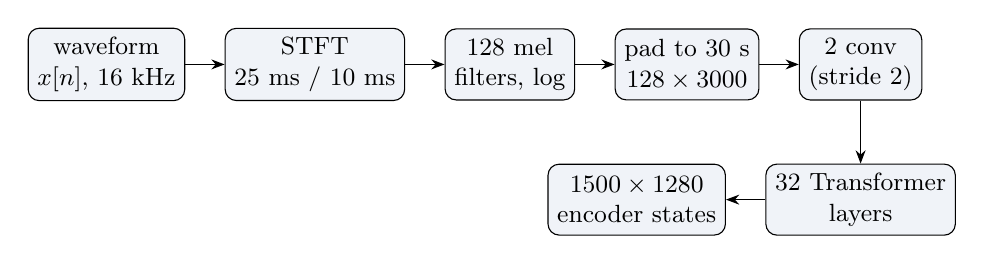
\begin{tikzpicture}[node distance=0.55cm and 0.5cm, every node/.style={font=\small},
  box/.style={draw, rounded corners, align=center, fill=defc!8, minimum height=0.9cm}]
\node[box] (wav) {waveform\\$x[n]$, 16 kHz};
\node[box, right=of wav] (stft) {STFT\\25 ms / 10 ms};
\node[box, right=of stft] (mel) {128 mel\\filters, log};
\node[box, right=of mel] (pad) {pad to 30 s\\$128\times3000$};
\node[box, right=of pad] (conv) {2 conv\\(stride 2)};
\node[box, below=0.8cm of conv] (enc) {32 Transformer\\layers};
\node[box, left=of enc] (out) {$1500\times1280$\\encoder states};
\draw[-Stealth] (wav)--(stft); \draw[-Stealth] (stft)--(mel); \draw[-Stealth] (mel)--(pad); \draw[-Stealth] (pad)--(conv);
\draw[-Stealth] (conv)--(enc); \draw[-Stealth] (enc)--(out);
\end{tikzpicture}
\caption{Whisper large-v3-turbo front end, from waveform to encoder states.}
\end{figure}

\begin{exercise}{A 27-second Telugu clip}{ex27}
How many valid encoder frames does it have, and how many \emph{text tokens} might it need if Telugu costs up to 45 Whisper tokens
per second?\par
\textit{Solution.} $T=\lfloor 50\cdot 27\rfloor+1=1351$. Text: up to $27\times 45=1215$ tokens, far above the decoder's 448-position
limit. Such an utterance cannot be transcribed in one pass; this is why training drops utterances over 440 text tokens and the demo
cuts audio into chunks of at most 12 s (Chapters~\ref{ch:whisper} and \ref{ch:demo}).
\end{exercise}

\chapter{Measuring Success: Edit Distance, WER, CER and LID Accuracy}
\chaptermark{Metrics}
\label{ch:metrics}

Before building anything we must agree on how to score it. A wrong metric would make every later comparison meaningless, and two
metric bugs in this project (Chapter~\ref{ch:lessons}) would have changed conclusions.

\section{Edit distance}

\begin{definition}{Levenshtein distance}{lev}
Let $\bm r=(r_1,\dots,r_n)$ and $\bm h=(h_1,\dots,h_m)$ be sequences over an alphabet. An \emph{edit} is one substitution
($r_i\to h_j$), deletion (drop $r_i$) or insertion (add $h_j$). The Levenshtein distance $d(\bm r,\bm h)$ is the minimum number of
edits that turns $\bm r$ into $\bm h$.
\end{definition}

\begin{theorem}{Dynamic programme for edit distance}{levdp}
Let $D[i,j]=d\big((r_1..r_i),(h_1..h_j)\big)$. Then $D[i,0]=i$, $D[0,j]=j$ and for $i,j\ge1$
\[
D[i,j]=\min\Big\{\,D[i-1,j]+1,\ \ D[i,j-1]+1,\ \ D[i-1,j-1]+\1[r_i\ne h_j]\,\Big\}.
\]
$d(\bm r,\bm h)=D[n,m]$, computed in $O(nm)$ time.
\end{theorem}
\begin{proof}
An optimal edit script, read left to right, aligns the prefixes. Look at its last operation. Either $r_i$ was deleted (cost 1 plus
the best way to turn $r_{1..i-1}$ into $h_{1..j}$), or $h_j$ was inserted (cost 1 plus $D[i,j-1]$), or $r_i$ was aligned with $h_j$
(cost 0 if equal, 1 if substituted, plus $D[i-1,j-1]$). Every script ends in one of these three ways, and each sub-problem is
solved optimally by induction on $i+j$, so the minimum of the three is optimal. The base cases need $i$ deletions or $j$ insertions.
\end{proof}

\begin{example}{``kitten'' $\to$ ``sitting''}{kitten}
\[
\begin{array}{c|cccccccc}
 & \epsilon & s & i & t & t & i & n & g\\\hline
\epsilon & 0&1&2&3&4&5&6&7\\
k & 1&\bm1&2&3&4&5&6&7\\
i & 2&2&\bm1&2&3&4&5&6\\
t & 3&3&2&\bm1&2&3&4&5\\
t & 4&4&3&2&\bm1&2&3&4\\
e & 5&5&4&3&2&\bm2&3&4\\
n & 6&6&5&4&3&3&\bm2&\bm3
\end{array}
\]
$d=3$: substitute $k\to s$, substitute $e\to i$, insert $g$. So $S=2$, $D=0$, $I=1$.
\end{example}

\section{WER and CER}

\begin{definition}{Word and character error rates}{wercer}
For a test set of utterances $i=1,\dots,K$ with references $\bm r^{(i)}$ and hypotheses $\bm h^{(i)}$, both \emph{normalised}
(Section~\ref{sec:norm}),
\[
\CER=\frac{\sum_{i} d_{\text{char}}\big(\bm r^{(i)},\bm h^{(i)}\big)}{\sum_i |\bm r^{(i)}|_{\text{char}}}
=\frac{S+D+I}{N},
\]
where sequences are compared character by character (spaces included). WER is the same with words (split on spaces) as symbols.
\end{definition}

Note the \emph{micro-average}: total errors over total reference length, not the mean of per-utterance rates. Long utterances weigh
more. This is what \texttt{jiwer.cer(list, list)} computes and what \file{metrics.py} reports.

\begin{proposition}{CER is not bounded by 1}{cerbound}
For one pair, $|m-n|\le d(\bm r,\bm h)\le\max(m,n)$. Hence $\CER\le\max(m,n)/n$, which is unbounded as $m\to\infty$.
\end{proposition}
\begin{proof}
Each edit changes the length by at most one, and the length must change by $|m-n|$, so $d\ge|m-n|$. Upper bound: substitute
$\min(m,n)$ aligned positions and insert or delete the remaining $|m-n|$ symbols, $\min(m,n)+|m-n|=\max(m,n)$ edits.
\end{proof}

\begin{intuition}[: what CER $>1$ means]
A CER above 1 means the hypothesis is much \emph{longer} than the reference. In this project it almost always means a
\emph{repetition loop}: the decoder keeps emitting the same phrase until it hits the 440-token limit. Vanilla Whisper's CER of
2.60 on IndicVoices Assamese is a loop symptom, not a ``very precise'' measure of quality.
\end{intuition}

\paragraph{Why CER is the primary metric here.}
\begin{itemize}
\item Indic words are long and inflected (Telugu is agglutinative): one wrong suffix makes the whole word wrong for WER, while CER
gives partial credit.
\item Spelling variation (e.g.\ with or without a nukta, two ways of writing a nasal) is common; CER penalises it by one character,
WER by a whole word.
\item Code-switched references write English words sometimes in Latin, sometimes in Indic script (Section~\ref{sec:csmetric}).
\end{itemize}
WER is still reported for completeness.

\section{Text normalisation}
\label{sec:norm}

Two strings that a human would call ``the same transcript'' can differ in Unicode bytes, punctuation and case. Scoring raw strings
would count these as errors. A \emph{single} normaliser is therefore applied to both the training targets and, at scoring time, to
both references and hypotheses.

\begin{definition}{The project's normaliser \file{normalize(text, lang)}}{normalizer}
\begin{enumerate}
\item Unicode NFC (canonical composition).
\item Delete bracketed spans: \texttt{<...>}, \texttt{[...]}, \texttt{(...)} (tags such as \texttt{<unintelligible>}).
\item Remove zero-width characters (ZWJ, ZWNJ, ZWSP, BOM).
\item For Indic languages: the IndicNLP normaliser of that language (canonical forms of nukta letters, chandrabindu, etc.).
\item For English: NFKC; keep in-word apostrophes, mapping the curly apostrophe U+2019 to \texttt{'}.
\item Lower-case.
\item Replace every Unicode \emph{symbol} (category S*) or \emph{punctuation} (category P*) character by a space. This includes the
danda \deva{।} (U+0964). Combining marks (category M*: matras, viramas) are \emph{kept}.
\item Collapse runs of whitespace; strip.
\end{enumerate}
Digits are \emph{not} converted to words.
\end{definition}

\begin{example}{Why NFC matters}{nfc}
The Devanagari letter \deva{क़} (qa) can be stored as one code point U+0958 or as two, \deva{क} U+0915 followed by the nukta U+093C.
They look identical, but a character-level comparison would count one substitution plus one insertion. NFC (plus IndicNLP's nukta
handling) maps both to the same sequence.
\end{example}

\begin{vivatip}[: two known side effects of the normaliser]
(1) Digits are not verbalised, so ``25'' vs ``twenty five'' counts as errors; this hurts Svarah (Chapter~\ref{ch:svarah}).
(2) Parenthesised text is deleted. For IndicVoices this removes tags, but in FLEURS the parenthesised words are usually \emph{read
aloud}, so 5--8\% of FLEURS rows lose spoken words from both targets and references. Re-scoring shows this inflates FLEURS CER by
0.005--0.02 for \emph{every} system (e.g.\ Stage 2 English 0.042 $\to$ 0.028 if kept). Rankings barely change. This was found in
the fourth code review and left open because fixing it changes the training targets.
\end{vivatip}

\section{LID metrics}

\begin{definition}{LID accuracy and confusion matrix}{lidacc}
For a test set whose true language is $\ell$, LID accuracy is the fraction of utterances with $\hat\ell=\ell$. Pooling all test sets,
the confusion matrix $C\in\mathbb N^{7\times7}$ has $C_{\ell\ell'}=\#\{\text{utterances of language }\ell\text{ predicted as }\ell'\}$.
Recall of $\ell$ is $C_{\ell\ell}/\sum_{\ell'}C_{\ell\ell'}$. \emph{Macro} accuracy averages per-set accuracies with equal weight.
\end{definition}

\section{Oracle versus predicted language}
\label{sec:oracle}

Whisper must be given a language token before it transcribes. We decode every test utterance twice:
\begin{itemize}
\item \textbf{Oracle LID}: the true language token is forced. This measures pure recognition quality.
\item \textbf{Predicted LID}: the model's own LID decision is used. This is what a user experiences.
\end{itemize}
The difference $\CER_{\text{pred}}-\CER_{\text{oracle}}$ is the \emph{routing cost} of LID errors. The literature reports about
4 CER points for a strong LID-then-ASR system (TalTech, ML-SUPERB 2.0); we measure ours in Chapter~\ref{ch:results}.

\begin{incode}
\file{eval_whisper.py} decodes with the oracle token, predicts the language, and \emph{re-decodes only the utterances whose
predicted language differs} (the same token gives the same greedy decode, so the oracle output is reused). It reports
\texttt{oracle\_norm}, \texttt{oracle\_raw}, \texttt{pred\_norm}, \texttt{lid\_acc}, \texttt{lid\_conf}, and the LID-head accuracy.
\end{incode}

\begin{exercise}{Micro vs macro}{micro}
Set A has 2 utterances: reference lengths 10 and 90 characters, with 5 and 9 errors. Compute the micro CER and the mean of per-utterance CERs.\par
\textit{Solution.} Micro: $(5+9)/(10+90)=0.14$. Mean of rates: $(0.5+0.1)/2=0.30$. The short utterance dominates the macro value.
The project uses micro CER within a test set, and reports the plain mean over test sets as the summary (``mean over 23 sets'').
\end{exercise}

\chapter{Sequence-to-Sequence Learning and the Transformer}
\chaptermark{Sequence-to-Sequence and Transformers}
\label{ch:seq2seq}

ASR maps a sequence (audio frames) to another sequence (text tokens) of a different, unknown length. This chapter derives the
standard tool for that, the encoder--decoder Transformer, at the level needed to understand every later chapter.

\section{Autoregressive factorisation}

Let $\vy=(y_1,\dots,y_U)$ be the target tokens, ending with an end-of-text token \tok{endoftext} (EOT). By the chain rule of
probability, \emph{any} distribution over sequences can be written as
\[
p_\theta(\vy\mid\vx)=\prod_{t=1}^{U}p_\theta(y_t\mid \vy_{<t},\vx).
\]
So it suffices to model one next-token distribution at a time. The decoder outputs logits $\vz_t\in\R^V$ and
$p_\theta(\cdot\mid\vy_{<t},\vx)=\softmax(\vz_t)$, where $\softmax(\vz)_v=e^{z_v}/\sum_{u}e^{z_u}$.

\begin{definition}{Maximum likelihood and token cross-entropy}{nll}
Given training pairs $(\vx^{(i)},\vy^{(i)})$, we minimise the negative log-likelihood, averaged over target tokens:
\[
\mathcal L_{\text{CE}}(\theta)=\frac{1}{\sum_i U_i}\sum_i\sum_{t=1}^{U_i}-\log p_\theta\big(y^{(i)}_t\mid \vy^{(i)}_{<t},\vx^{(i)}\big).
\]
\end{definition}

\begin{proposition}{Gradient of softmax cross-entropy}{cegrad}
For one position with logits $\vz$ and target $y$, $\ell(\vz)=-\log\softmax(\vz)_y$ has gradient $\nabla_{\vz}\ell=\bm p-\bm e_y$,
where $\bm p=\softmax(\vz)$ and $\bm e_y$ is the one-hot vector of $y$.
\end{proposition}
\begin{proof}
$\ell=-z_y+\log\sum_u e^{z_u}$. Then $\partial\ell/\partial z_v=-\1[v=y]+e^{z_v}/\sum_u e^{z_u}=p_v-\1[v=y]$.
\end{proof}

\begin{intuition}
The gradient pushes the correct logit up by $1-p_y$ and every wrong logit down by its own probability. Every token in the vocabulary
receives a gradient at every position. This matters in Chapter~\ref{ch:odia}: the new Odia token is pushed down at every position
of every non-Odia utterance, and up only where it is the target.
\end{intuition}

\section{Teacher forcing}

During training the decoder is fed the \emph{true} previous tokens, not its own predictions (``teacher forcing''). In practice the
decoder input is the target sequence shifted right by one, with a start token in front:
\[
\text{decoder input}=(\texttt{SOT},y_1,\dots,y_{U-1}),\qquad \text{labels}=(y_1,\dots,y_U).
\]
All $U$ positions are then computed in one parallel forward pass (with a causal mask, below). Positions that should not be
trained get the label $-100$, which PyTorch's cross-entropy ignores.

\section{Attention}

\begin{definition}{Scaled dot-product attention}{attn}
Given queries $Q\in\R^{n\times d_k}$, keys $K\in\R^{m\times d_k}$ and values $V\in\R^{m\times d_v}$,
\[
\mathrm{Attn}(Q,K,V)=\softmax\!\Big(\frac{QK^\top}{\sqrt{d_k}}+M\Big)V,
\]
with the softmax taken row by row and $M$ a mask ($0$ = allowed, $-\infty$ = forbidden). Row $i$ of the output is a convex
combination of the value vectors, weighted by how well query $i$ matches each key.
\end{definition}

\begin{proposition}{Why divide by $\sqrt{d_k}$}{scale}
If the entries of $\bm q,\bm k\in\R^{d_k}$ are independent with mean 0 and variance 1, then $\E[\bm q^\top\bm k]=0$ and
$\mathrm{Var}(\bm q^\top\bm k)=d_k$. Dividing by $\sqrt{d_k}$ restores unit variance.
\end{proposition}
\begin{proof}
$\bm q^\top\bm k=\sum_{j}q_jk_j$. Each term has mean $\E q_j\E k_j=0$ and variance $\E[q_j^2]\E[k_j^2]=1$, and the terms are
independent, so variances add to $d_k$.
\end{proof}
Without the scaling, large dot products saturate the softmax (almost one-hot), whose gradients are then nearly zero.

\paragraph{Multi-head attention.} The model dimension $d$ is split into $H$ heads of size $d/H$. Each head has its own
projections $W^Q_h,W^K_h,W^V_h\in\R^{d\times d/H}$; the head outputs are concatenated and multiplied by $W^O\in\R^{d\times d}$. In
HuggingFace's Whisper these four matrices are the modules \texttt{q\_proj}, \texttt{k\_proj}, \texttt{v\_proj}, \texttt{out\_proj}:
exactly the names LoRA targets in Chapter~\ref{ch:lora}.

\paragraph{Three kinds of attention in an encoder--decoder.}
\begin{enumerate}
\item \textbf{Encoder self-attention}: queries, keys and values all come from the encoder; no mask (every frame sees every frame).
\item \textbf{Decoder causal self-attention}: from the decoder; $M_{ij}=-\infty$ for $j>i$, so position $i$ cannot look at
future tokens. This is what makes parallel teacher-forced training equivalent to left-to-right generation.
\item \textbf{Cross-attention}: queries from the decoder, keys and values from the encoder output. This is how the text ``reads''
the audio.
\end{enumerate}

\section{The Transformer block}

Whisper uses \emph{pre-norm} residual blocks. For an encoder layer with input $H\in\R^{n\times d}$:
\[
H\leftarrow H+\mathrm{MHA}(\LN(H)),\qquad H\leftarrow H+\mathrm{MLP}(\LN(H)),\qquad
\mathrm{MLP}(\bm u)=W_2\,\mathrm{GELU}(W_1\bm u+\bm b_1)+\bm b_2,
\]
with $W_1\in\R^{4d\times d}$ (\texttt{fc1}) and $W_2\in\R^{d\times 4d}$ (\texttt{fc2}). A decoder layer has three sub-blocks:
causal self-attention, cross-attention, MLP. Positional information is added at the input (sinusoidal for the encoder, learned for
the decoder), because attention itself is permutation-invariant.

\begin{intuition}[: residual streams]
Each block \emph{adds} a correction to a running ``residual stream''. If a block's output is zero, the layer is the identity. This is
exactly why LoRA can be initialised so that the fine-tuned model starts identical to the pretrained one: an added correction of zero
changes nothing (Chapter~\ref{ch:lora}).
\end{intuition}

\section{Decoding}

At inference time there is no reference, so tokens are generated one by one. This project uses \textbf{greedy decoding}:
$\hat y_t=\argmax_v p_\theta(v\mid\hat{\vy}_{<t},\vx)$ until EOT or a maximum of 440 new tokens.

\paragraph{KV cache.} At step $t$ the keys and values of positions $1..t-1$ do not change, so they are cached; each step computes
only the new position. Generating $U$ tokens costs $O(U)$ decoder passes of one position each instead of $O(U^2)$ total positions.
The encoder runs once per clip.

\begin{exercise}{Why is training parallel but inference sequential?}{par}
\textit{Solution.} In training all inputs $(\texttt{SOT},y_1,\dots,y_{U-1})$ are known in advance (teacher forcing), and the causal
mask guarantees position $t$ uses only positions $<t$, so all positions are computed at once. In inference $\hat y_t$ is needed to
compute position $t+1$, so steps must run one after another.
\end{exercise}

\begin{vivatip}
A classic question: ``what is exposure bias?'' With teacher forcing the decoder never sees its own mistakes during training; at test
time one wrong token can push it into states it never saw. Repetition loops are one visible symptom. The hard 440-token cap and the
``loop rate'' metric (fraction of outputs that hit the cap) are the project's guards.
\end{vivatip}

\chapter{Whisper: Architecture, Tokenizer, Prompt and Built-in LID}
\chaptermark{Whisper}
\label{ch:whisper}

\section{What Whisper is}

Whisper (Radford et al., 2023) is an encoder--decoder Transformer (Chapter~\ref{ch:seq2seq}) trained by OpenAI on about 680{,}000
hours of weakly labelled web audio in about 100 languages. It does transcription, translation to English, timestamps and language
identification, all through the decoder's token stream.

\begin{center}
\begin{tabular}{lccc}
\toprule
 & Whisper-small & large-v3 & \textbf{large-v3-turbo} (our base)\\
\midrule
Parameters & 244 M & 1.55 B & 809 M\\
Encoder layers & 12 & 32 & 32\\
Decoder layers & 12 & 32 & \textbf{4}\\
Width $d$ / heads & 768 / 12 & 1280 / 20 & 1280 / 20\\
MLP width & 3072 & 5120 & 5120\\
Mel bins $M$ & 80 & 128 & 128\\
Vocabulary $V$ & 51{,}865 & 51{,}866 & 51{,}866\\
Max decoder positions & 448 & 448 & 448\\
\bottomrule
\end{tabular}
\end{center}

\emph{Turbo} is large-v3 with the decoder pruned from 32 to 4 layers and then fine-tuned further. Generation runs one decoder pass
per token, so a 4-layer decoder makes decoding about 6 times faster, while the large 32-layer encoder keeps most of the acoustic
quality. Whisper-small was the development model for experiments E1--E4 (Chapter~\ref{ch:results}); turbo is the final model.

\section{Byte-level BPE and why Indic text is expensive}

\begin{definition}{Byte-level byte-pair encoding (BPE)}{bpe}
Text is first written as UTF-8 bytes (256 base symbols). BPE training repeatedly finds the most frequent adjacent pair of symbols in a
training corpus and merges it into a new symbol, until the vocabulary has the desired size. Tokenising a new string applies the
learned merges greedily. Any string can be tokenised (in the worst case one token per byte).
\end{definition}

UTF-8 encodes an ASCII letter in 1 byte and a character of an Indic script in 3 bytes. Whisper's merges were learned mostly from
English-heavy text, so frequent English words become single tokens, while Indic text is split into short pieces, often single
characters or bytes.

\begin{example}{Token cost measured on our data}{tokcost}
Measured with \file{prep_tokens.py} on the normalised transcripts: Indic speech costs \textbf{17--45 Whisper tokens per second}, English
about 3. Of Telugu, Assamese and Bengali reference transcripts, 41--58\% exceed 200 tokens, and some exceed 448, the decoder's
hard limit.
\end{example}

\begin{proposition}{Token budget}{budget}
The decoder sequence has at most 448 positions. Our prompt uses 4 (Section~\ref{sec:prompt}) and the target ends with EOT. So a
transcript can be learned in one pass only if it has at most $448-4-1=443$ text tokens. The project uses 440, leaving a small margin.
\end{proposition}

\begin{incode}
\file{common.py: MAX_TEXT_TOKENS = 440}. Training drops utterances with more than 440 text tokens (8{,}131 utterances, 2.1\% of
the training split). Test keeps everything; the 550 over-budget test utterances simply count as errors (they cannot be completed).
All decoding uses \texttt{max\_new\_tokens=440}. The first baseline run used 200, which truncated Indic outputs (bug 5).
\end{incode}

\section{The prompt and special tokens}
\label{sec:prompt}

Whisper's decoder is conditioned by special tokens. For plain transcription without timestamps the sequence is
\[
\underbrace{\texttt{SOT}}_{\text{start}}\ \ \underbrace{\tok{hi}}_{\text{language}}\ \ \tok{transcribe}\ \ \tok{notimestamps}\ \
\text{text tokens}\ \dots\ \ \texttt{EOT}.
\]

\begin{definition}{The project's training sequence}{trainseq}
For an utterance of language $\ell$ with text tokens $w_1..w_K$:
\begin{align*}
\text{decoder input}&=[\texttt{SOT},\ \tok{$\ell$},\ \tok{transcribe},\ \tok{notimestamps},\ w_1,\dots,w_K]\\
\text{labels}&=[\tok{$\ell$},\ \tok{transcribe},\ \tok{notimestamps},\ w_1,\dots,w_K,\ \texttt{EOT}]
\end{align*}
The first label is the language token: \textbf{the language is a supervised target}, predicted from \texttt{SOT} and the audio alone.
\end{definition}

The usual HuggingFace recipe puts the language in the \emph{forced} prefix, so the model is told the language and never learns to
predict it. That is the documented cause of LID collapse after fine-tuning. Making it a label keeps LID trained.

\section{Built-in language identification}

\begin{definition}{Closed-set decoder-token LID}{tokenlid}
Feed only $[\texttt{SOT}]$ to the decoder. Let $\vz_1$ be the logits of the first predicted position. Restrict to the language
tokens of $\mathcal L$:
\[
\hat p_{\text{tok}}(\ell\mid\vx)=\frac{\exp z_{1,\mathrm{id}(\ell)}}{\sum_{\ell'\in\mathcal L}\exp z_{1,\mathrm{id}(\ell')}},
\qquad \hat\ell=\argmax_{\ell\in\mathcal L}\hat p_{\text{tok}}(\ell\mid\vx).
\]
\end{definition}

This is a closed-set softmax over 7 of the $\approx$51{,}867 logits. Vanilla Whisper's version of this collapses outside
English and Hindi on our test data: Telugu 14\%, Assamese 0\%, Bengali 51\%, Marathi 52\% (Chapter~\ref{ch:results}).

\begin{vivatip}[: Odia]
Whisper's 100 languages do \emph{not} include Odia. This was checked three ways: the official \file{whisper/tokenizer.py}, the HF
\texttt{generation\_config.lang\_to\_id} (100 entries, no \texttt{or} or \texttt{od}), and the vocabulary itself. So for vanilla
Whisper, Odia cannot be predicted or forced at all, and Odia CER is above 1 (it writes Odia speech in other scripts or loops).
\end{vivatip}

\section{Baseline numbers that motivated the project}

Zero-shot test CER (100 utterances per set, mean over non-code-switched corpora of each language; \file{reports/baselines/summary.md}):

\begin{center}
\begin{tabular}{lcccc}
\toprule
Language & Whisper-small & Whisper-turbo & IndicConformer-600M & Turbo LID accuracy\\
\midrule
English & 0.04 & 0.03 & n/a & 100\%\\
Hindi & 1.09 & 0.21 & 0.05 & 81\%\\
Marathi & 1.13 & 0.40 & 0.05 & 52\%\\
Bengali & 1.68 & 0.72 & 0.05 & 51\%\\
Telugu & 2.11 & 0.66 & 0.07 & 14\%\\
Assamese & 1.58 & 1.90 & 0.06 & 0\%\\
Odia & 1.66 & 1.46 & 0.07 & no token\\
\bottomrule
\end{tabular}
\end{center}

Vanilla Whisper is usable only for English and Hindi. IndicConformer (an Indic-specialised Conformer trained on AI4Bharat data) is far
better on Indic CER but has no English and no LID. The project's aim is to close as much of this gap as possible \emph{inside one
model that also does English, code-switching and LID}.

\begin{exercise}{Why does a 4-layer decoder hardly hurt accuracy?}{turbo}
\textit{Solution.} In ASR most of the work is acoustic: deciding which sounds were spoken. That is done by the encoder, which is
kept at 32 layers. The decoder mainly acts as a conditional language model that reads the encoder through cross-attention; a shallow
decoder is enough for that. Since generation cost is proportional to decoder depth times number of tokens, cutting the decoder
gives the speed-up for little accuracy loss.
\end{exercise}

\chapter{Data: Corpora, Pipeline, and Honest Train/Test Splits}
\chaptermark{Data and Splits}
\label{ch:data}

\section{The corpora}

\begin{center}
\small
\begin{tabularx}{\linewidth}{lYYl}
\toprule
Corpus & Languages & Character & Role\\
\midrule
IndicVoices (AI4Bharat) & as, bn, hi, mr, or, te & spontaneous, many speakers, the hardest & train / dev / test\\
Kathbath (AI4Bharat) & bn, hi, mr, or, te (no as) & read sentences, phone recordings & train / dev / test\\
Shrutilipi & as, bn, hi, mr, or, te & All India Radio news, read & train only\\
FLEURS (Google) & all 7 & read Wikipedia sentences & train / dev / test\\
LibriSpeech & en & read audiobooks (clean-100, dev/test-clean) & train / dev / test\\
MUCS 2021 & hi--en, bn--en & code-switched lectures & train / dev / test\\
Svarah & en (Indian accent) & 117 speakers, 65 districts & test only\\
Lahaja & hi (many accents) & multi-accent Hindi & test only\\
MUSAN (noise, music), RIRs & -- & augmentation and robustness tests & 80\% train / 20\% eval\\
\bottomrule
\end{tabularx}
\end{center}

Training hours per language after splitting (from \file{reports/splits.txt}):

\begin{center}
\small
\begin{tabular}{lrrrrrr}
\toprule
 & FLEURS & IndicVoices & Kathbath & Shrutilipi & LibriSpeech & MUCS (code-switch)\\
\midrule
hi & 6.6 & 55.5 & 14.1 & 21.0 & -- & 77.6\\
mr & 11.8 & 48.2 & 13.6 & 22.2 & -- & --\\
bn & 10.6 & 44.6 & 13.3 & 21.0 & -- & 40.0\\
as & 10.4 & 54.0 & -- & 23.9 & -- & --\\
or & 3.4 & 54.7 & 13.4 & 24.7 & -- & --\\
te & 7.9 & 49.4 & 14.6 & 21.9 & -- & --\\
en & 7.4 & -- & -- & -- & 100.6 & --\\
\bottomrule
\end{tabular}
\end{center}

These are the \emph{downloaded subsets} (some shards of each corpus), chosen so that every language has roughly 85--110 hours.

\section{The pipeline}

\begin{enumerate}
\item \file{audit_data.py}: reads only metadata and writes hours, utterances and speakers per corpus, language and split to
\file{reports/data_audit.csv}.
\item \file{build_manifests.py}: decodes every corpus to 16 kHz mono FLAC and writes one JSON line per utterance:
\texttt{id, corpus, lang, split, path, dur, text, text\_norm, speaker, cs}. It drops clips longer than 30 s (they do not fit
Whisper's window), shorter than 0.3 s, or with an empty normalised text. MUCS long recordings are cut using its \texttt{segments}
file. Result: 467{,}515 utterances.
\item \file{make_splits.py}: assigns each utterance to train, dev or test (next section).
\item \file{prep_tokens.py}: adds \texttt{ntok}, the Whisper token count of \texttt{text\_norm}.
\item \file{balanced_mix.py}: builds the 700-hour training mix (Chapter~\ref{ch:balance}).
\end{enumerate}

\section{Why the split must be speaker-disjoint}

\begin{definition}{Generalisation error}{generr}
Let $\mathcal D$ be the distribution of (audio, transcript) pairs a deployed system will meet, and $\ell$ a loss. The quantity we
want is $R(h)=\E_{(\vx,\vy)\sim\mathcal D}[\ell(h(\vx),\vy)]$. A test set estimates $R(h)$ by an average
$\hat R(h)=\frac1K\sum_{i}\ell(h(\vx_i),\vy_i)$, which is unbiased only if the test pairs are drawn from $\mathcal D$
\emph{independently of the training data}.
\end{definition}

A real user is (almost always) a \emph{new speaker}. If test speakers also appear in training, the model may have memorised their
voice, accent and microphone, and $\hat R$ underestimates $R$. The test pairs are then not independent of the training sample.

\begin{example}{The official splits were not speaker-disjoint}{spk}
\file{make_splits.py} checks the official IndicVoices and Kathbath \texttt{train} vs \texttt{valid} splits:
\begin{center}
\begin{tabular}{lccc}
\toprule
Corpus & train speakers & valid speakers & shared\\
\midrule
IndicVoices & 4{,}915 & 2{,}702 & \textbf{1{,}217}\\
Kathbath & 170 & 91 & \textbf{40}\\
\bottomrule
\end{tabular}
\end{center}
Fix: every \texttt{valid} utterance whose speaker occurs in \texttt{train} is moved to train. Dev and test are drawn only from
valid-only speakers (30\% of those speakers to dev, the rest to test). The script then re-checks: train$\cap$dev $=$
train$\cap$test $=$ dev$\cap$test $=\emptyset$ for IndicVoices, Kathbath and MUCS.
\end{example}

\paragraph{Role assignment per corpus.}
\begin{itemize}
\item IndicVoices, Kathbath: as above.
\item Shrutilipi: train only (no speaker ids exist, so a speaker-disjoint test split is impossible).
\item FLEURS, LibriSpeech: their official train/dev/test (already speaker-disjoint by construction).
\item MUCS: official test is test; 5\% of training \emph{recordings} go to dev (recording ids act as speakers).
\item Svarah, Lahaja: test only.
\end{itemize}

\section{Text leakage}

Many corpora reuse sentences: different speakers read the same prompt. If a test sentence's text is in training, the decoder may
recall it as a language model rather than recognise it.

\begin{definition}{Leakage removal}{leak}
For each language $\ell$, let $\mathcal T_\ell$ be the set of normalised texts of all dev and test utterances of $\ell$. Every training
utterance of $\ell$ whose normalised text is in $\mathcal T_\ell$ is removed (\texttt{role = dropped\_leak}).
\end{definition}

Removed: IndicVoices hi 5{,}005, mr 2{,}862, or 2{,}667, te 2{,}042, bn 2{,}036, as 1{,}357; MUCS hi 4{,}964, bn 2{,}538; a handful in
LibriSpeech and Shrutilipi. (MUCS lectures repeat phrases often, hence the large count.)

\begin{center}
\fbox{\parbox{0.8\linewidth}{\centering Final split: \textbf{384{,}027 train} / \textbf{14{,}883 dev} / \textbf{45{,}104 test} utterances.}}
\end{center}

\section{Unique ids}

Bug 8: 19{,}361 ids were not unique (FLEURS sentence ids are shared by several speakers; some shards had identical file names in
every language). Paths were always unique, so no audio was lost, but ids are used to pair hypotheses across systems in the
statistics of Chapter~\ref{ch:eval}, so they were made unique and the splits regenerated.

\begin{exercise}{Why is Shrutilipi train-only, and why does that not bias the results?}{shru}
\textit{Solution.} It has no speaker labels, so we cannot guarantee that a Shrutilipi test speaker is unseen. Using it only for
training is safe: the speakers of the other corpora's test sets are a different population (AI4Bharat recruits vs radio
newsreaders), and none of our test sets is drawn from Shrutilipi.
\end{exercise}

\begin{vivatip}
If an examiner asks ``how do you know your numbers are not inflated?'', the three checks are: speaker-disjoint dev/test (re-verified
with 0 overlap), text-leakage removal, and test sets never used for any decision (E1--E4 used the dev split only; the test split was
used once, for the final model and baselines). The one exception is calibration of the LID rule on Svarah, which used a
\emph{speaker-disjoint} Svarah subset (Chapter~\ref{ch:svarah}).
\end{vivatip}

\chapter{Balanced Sampling: Giving Every Language a Fair Share}
\chaptermark{Balanced Sampling}
\label{ch:balance}

\section{Why the mix matters: the objective is a weighted sum}

Let the training mix sample language $\ell$ with probability $\pi_\ell$, and let $R_\ell(\theta)$ be the expected per-token loss on
language $\ell$. The expected mini-batch loss that SGD minimises is
\[
\E[\mathcal L_{\text{batch}}(\theta)]\approx\sum_{\ell\in\mathcal L}\pi_\ell\,R_\ell(\theta),
\qquad
\E[\nabla\mathcal L_{\text{batch}}]\approx\sum_\ell\pi_\ell\nabla R_\ell(\theta).
\]
(``$\approx$'' because the loss is averaged over tokens, and languages differ in tokens per utterance.)

\begin{proposition}{The mix chooses the objective}{mixobj}
Training on a mix with weights $\pi$ minimises the $\pi$-weighted risk $\sum_\ell\pi_\ell R_\ell$. If we report results as a plain
average over languages, the matching training objective is $\pi_\ell=1/|\mathcal L|$.
\end{proposition}
\begin{proof}
Immediate from linearity of expectation over the sampling of the language of each example.
\end{proof}

With natural proportions ($\pi_\ell\propto$ hours available), a language with 5\% of the data gets 5\% of the gradient. Its errors
barely move the objective, so the model under-fits it. The price of equalising is repetition: a small corpus is seen several times
per epoch, which risks over-fitting. The design below caps that repetition.

\section{The two-stage algorithm}

\begin{definition}{Two-stage deterministic balanced upsampling (Polyglot-Lion style)}{twostage}
Constants: $T_h=90$ hours per language, replication cap $\rho=3$, share cap $\kappa=0.7$, code-switch fraction $f=0.1$.

\textbf{Stage 1 (within a language).} Let $h_c$ be the hours of corpus $c$ for this language and $h_{\max}=\max_c h_c$. Set
\[
s_c=h_c\cdot\min\!\Big(\rho,\ \frac{h_{\max}}{h_c}\Big),\qquad \text{share}_c=\frac{s_c}{\sum_{c'}s_{c'}}.
\]
If some shares exceed $\kappa$, set those to $\kappa$ and rescale the others to fill $1-\kappa\cdot\#\text{capped}$ (repeat up to 10
times; skipped if every corpus is over the cap).

\textbf{Stage 2 (across languages).} Corpus $c$ contributes exactly $T_h\cdot\text{share}_c$ hours: $\lfloor\text{target}/h_c\rfloor$
full copies plus a seeded random subset for the remainder (fewer than one copy means sub-sampling).

\textbf{Code-switch pool.} MUCS gets $\frac{f}{1-f}\cdot|\mathcal L|\,T_h$ hours, split 60\% Hindi--English, 40\% Bengali--English.
\end{definition}

Stage 1 says: \emph{inside} a language, small corpora are pulled up toward the largest, but never replicated more than 3 times, and
no single corpus may take more than 70\% of the language (so the language keeps several domains: read, spontaneous, news).

\begin{proposition}{Total size of the mix}{mixsize}
The mix has $|\mathcal L|T_h/(1-f)$ hours, of which a fraction $f$ is code-switched. With 7 languages, $T_h=90$, $f=0.1$:
$630+70=\mathbf{700}$ hours.
\end{proposition}
\begin{proof}
Monolingual: $|\mathcal L|T_h$. Code-switch: $\frac{f}{1-f}|\mathcal L|T_h$. Sum: $|\mathcal L|T_h\big(1+\frac{f}{1-f}\big)=
\frac{|\mathcal L|T_h}{1-f}$. Its code-switch fraction is $\frac{f}{1-f}\big/\frac{1}{1-f}=f$.
\end{proof}

\begin{example}{Hindi}{mixhi}
$h$: FLEURS 6.6, IndicVoices 55.5, Kathbath 14.1, Shrutilipi 21.0; $h_{\max}=55.5$.
\begin{center}
\begin{tabular}{lcccccc}
\toprule
Corpus & $h_c$ & $h_{\max}/h_c$ & $s_c$ & share & target (h) & replication\\
\midrule
FLEURS & 6.6 & 8.41 & 19.8 & 0.114 & 10.3 & 1.56$\times$\\
IndicVoices & 55.5 & 1.00 & 55.5 & 0.321 & 28.9 & 0.52$\times$\\
Kathbath & 14.1 & 3.94 & 42.3 & 0.244 & 22.0 & 1.56$\times$\\
Shrutilipi & 21.0 & 2.64 & 55.5 & 0.321 & 28.9 & 1.37$\times$\\
\midrule
Sum & 97.2 & & 173.1 & 1.000 & 90.0 & \\
\bottomrule
\end{tabular}
\end{center}
No share exceeds 0.7. IndicVoices is \emph{sub-sampled} to about half per epoch, while FLEURS and Kathbath are repeated. (The real
run uses hours after the 440-token filter, so its numbers differ slightly.)
\end{example}

\begin{example}{English: the share cap in action}{mixen}
$h$: FLEURS 7.4, LibriSpeech 100.6. Stage 1: $s=(3\cdot7.4,\ 100.6)=(22.2,\ 100.6)$, shares $(0.181,\ 0.819)$. LibriSpeech exceeds
$\kappa=0.7$, so it is capped at 0.7 and FLEURS gets $0.3$. Targets: FLEURS $27$ h, i.e.\ \textbf{3.65$\times$} replication
(the share cap overrides the replication cap; the log notes ``English FLEURS replicated 3.6$\times$''), LibriSpeech 63 h.
\end{example}

\begin{exercise}{Odia FLEURS}{mixor}
Odia: FLEURS 3.4, IndicVoices 54.7, Kathbath 13.4, Shrutilipi 24.7 hours. Find FLEURS's target hours.\par
\textit{Solution.} $h_{\max}=54.7$. $s$: FLEURS $3\cdot3.4=10.2$; IndicVoices $54.7$; Kathbath $3\cdot13.4=40.2$; Shrutilipi
$24.7\cdot\min(3,2.21)=54.7$. Sum $159.8$. FLEURS share $10.2/159.8=0.064$, target $5.7$ h ($1.69\times$).
\end{exercise}

\paragraph{The result.} One deterministic file, \file{splits/train_mix_epoch0.jsonl}: 349{,}592 utterance references (no audio is
copied), exactly 90 h per language plus 70 h of code-switch (42 h hi--en, 28 h bn--en). Language tags are kept, because they are
needed as the \tok{$\ell$} target and the LID-CTC target. (Polyglot-Lion drops tags so the model learns LID implicitly; we need an
explicit LID output, so we keep them.)

\begin{intuition}[: deterministic vs temperature sampling]
The classical alternative samples language $\ell$ with $\pi_\ell\propto n_\ell^{1/\tau}$ (temperature $\tau$). It works but $\tau$
is a sensitive knob and the realised hours per language are random. The two-stage method gives exactly equal hours by construction.
\end{intuition}

\section{Evidence: experiment E3}

Whisper-small, LoRA, Hindi/Telugu/Assamese with a deliberately skewed pool (hi 97 h, te 26 h, as 5 h), same number of steps. Dev CER:

\begin{center}
\begin{tabular}{lcccc}
\toprule
Set & unbalanced & balanced & change\\
\midrule
FLEURS as & 0.242 & \textbf{0.182} & $-0.060$\\
IndicVoices as & 0.342 & \textbf{0.278} & $-0.064$\\
FLEURS te & 0.129 & 0.119 & $-0.010$\\
FLEURS hi & \textbf{0.096} & 0.111 & $+0.015$\\
IndicVoices hi & \textbf{0.097} & 0.113 & $+0.016$\\
\bottomrule
\end{tabular}
\end{center}

Exactly what Proposition~\ref{prop:mixobj} predicts: the scarcest language (Assamese) gains a lot, the richest (Hindi) loses a
little. Decision: balance.

\begin{incode}
\file{balanced_mix.py}: \texttt{corpus\_shares} (Stage 1 with the cap loop), \texttt{take} (full copies + seeded remainder),
\texttt{build} (Stage 2 + code-switch). Run \texttt{python balanced\_mix.py 1} to get a reshuffled second epoch. Bug 23: a language
with a single corpus would have been capped at 70\% of $T_h$; fixed by skipping the cap when every corpus is over it.
\end{incode}

\begin{vivatip}
Note what one epoch of this mix means for IndicVoices: it is sub-sampled to 0.5--0.7$\times$ per epoch. Stage 2 trained exactly one
epoch of mix 0, so part of the IndicVoices training data was never seen. A second epoch should use a reseeded mix (seed 1), not
mix 0 again.
\end{vivatip}

\chapter{Parameter-Efficient Fine-Tuning with LoRA}
\chaptermark{LoRA}
\label{ch:lora}

\section{The problem with full fine-tuning}

Full fine-tuning updates all 809 M parameters of turbo. AdamW stores two extra numbers per parameter (first and second moments),
plus gradients, so memory is several times the model size. It also lets the model drift far from what it learned on 680{,}000 hours,
which risks \emph{catastrophic forgetting} and over-fitting a few hundred hours.

\section{Low-rank adaptation}

\begin{definition}{LoRA (Hu et al., 2021)}{lora}
Take a frozen linear layer $\bm u\mapsto W_0\bm u$ with $W_0\in\R^{d_{\text{out}}\times d_{\text{in}}}$. LoRA replaces it by
\[
\bm u\ \mapsto\ W_0\bm u+\frac{\alpha}{r}\,B A\bm u,\qquad A\in\R^{r\times d_{\text{in}}},\ B\in\R^{d_{\text{out}}\times r},\ r\ll\min(d_{\text{in}},d_{\text{out}}).
\]
Only $A$ and $B$ are trained. Initialisation: $A$ random (Kaiming-uniform), $B=0$. Dropout (here 0.05) is applied to $\bm u$ on the
LoRA branch only.
\end{definition}

\begin{proposition}{Properties of LoRA}{loraprops}
\begin{enumerate}
\item At initialisation the model is exactly the pretrained model.
\item The update $\Delta W=\frac{\alpha}{r}BA$ has $\rank\Delta W\le r$.
\item It needs $r(d_{\text{in}}+d_{\text{out}})$ trainable numbers instead of $d_{\text{in}}d_{\text{out}}$.
\item After training it can be merged, $W=W_0+\frac\alpha rBA$, so inference costs exactly the same as the original model.
\end{enumerate}
\end{proposition}
\begin{proof}
(1) $B=0\Rightarrow\Delta W=0$. (2) $\mathrm{range}(BA)\subseteq\mathrm{range}(B)$, which has dimension at most $r$.
(3) Count entries of $A$ and $B$. (4) $W_0\bm u+\frac\alpha rBA\bm u=(W_0+\frac\alpha rBA)\bm u$ by linearity.
\end{proof}

\begin{proposition}{Gradients and the ``B moves first'' effect}{loragrad}
Let $\bm g=\partial\mathcal L/\partial\bm o$ be the gradient at the layer output $\bm o=W_0\bm u+\frac\alpha rBA\bm u$. Then
\[
\frac{\partial\mathcal L}{\partial B}=\frac\alpha r\,\bm g\,(A\bm u)^\top,\qquad
\frac{\partial\mathcal L}{\partial A}=\frac\alpha r\,B^\top\bm g\,\bm u^\top .
\]
At initialisation ($B=0$) the gradient with respect to $A$ is zero, and only $B$ changes in the first step.
\end{proposition}
\begin{proof}
$\bm o$ depends on $B$ through $\frac\alpha r B\bm v$ with $\bm v=A\bm u$; $\partial(\bm g^\top B\bm v)/\partial B=\bm g\bm v^\top$.
Similarly $\bm g^\top BA\bm u=(B^\top\bm g)^\top A\bm u$ gives $\partial/\partial A=B^\top\bm g\,\bm u^\top$. With $B=0$ this vanishes.
\end{proof}

\begin{intuition}[: why low rank is enough]
Adapting a pretrained model to a related task seems to need only a few new ``directions'' in each layer: the pretrained features are
already rich. The ratio $\alpha/r$ fixes the scale of the update so that changing $r$ does not require re-tuning the learning rate.
Here $\alpha/r=64/32=2$.
\end{intuition}

\section{Where LoRA goes, and the exact parameter count}

LoRA is applied to every attention projection (\texttt{q\_proj, k\_proj, v\_proj, out\_proj}) and both MLP matrices (\texttt{fc1,
fc2}) in every encoder and decoder layer, with $r=32$, $\alpha=64$. In addition the bottom third of encoder layers is frozen:
$\lfloor 32\times0.33\rfloor=10$ layers, so their LoRA matrices are not trained either (lower encoder layers are largely
language-independent acoustic feature extractors; freezing them reduces over-fitting).

\begin{example}{Counting the 86{,}880{,}008 ``trainable'' parameters of Stage 2}{count}
Turbo: $d=1280$, MLP width $5120$. One LoRA pair on a $d_{\text{out}}\times d_{\text{in}}$ matrix costs $32(d_{\text{in}}+d_{\text{out}})$.
\begin{itemize}
\item Attention projection ($1280\to1280$): $32\cdot2560=81{,}920$.\quad \texttt{fc1} or \texttt{fc2}: $32\cdot(1280+5120)=204{,}800$.
\item Encoder layer: $4\cdot81{,}920+2\cdot204{,}800=737{,}280$. Trainable encoder layers: $32-10=22$, giving $16{,}220{,}160$.
\item Decoder layer: self-attention and cross-attention ($8$ projections) $+$ MLP: $8\cdot81{,}920+2\cdot204{,}800=1{,}064{,}960$.
Four layers: $4{,}259{,}840$.
\item LoRA total: $\mathbf{20{,}480{,}000}$.
\item Embedding matrix with the Odia row: $51{,}867\times1280=66{,}389{,}760$ (counted because \texttt{requires\_grad=True}, although a
gradient mask lets only one row of 1{,}280 numbers change; Chapter~\ref{ch:odia}).
\item LID-CTC head: $1280\times8+8=10{,}248$.
\end{itemize}
Sum: $20{,}480{,}000+66{,}389{,}760+10{,}248=86{,}880{,}008$, exactly the 86.9 M printed in the training log. The parameters that
\emph{actually} change are $20{,}480{,}000+1{,}280+10{,}248\approx$ \textbf{20.5 M}, about 2.5\% of the model.
\end{example}

\begin{exercise}{Whisper-small's 13.0 M}{countsmall}
Whisper-small: $d=768$, MLP $3072$, 12 encoder and 12 decoder layers, nothing frozen. Verify the 13.0 M trainable parameters of E1.\par
\textit{Solution.} Attention pair: $32\cdot1536=49{,}152$; MLP pair: $32\cdot3840=122{,}880$. Encoder layer:
$4\cdot49{,}152+2\cdot122{,}880=442{,}368$; decoder layer: $8\cdot49{,}152+2\cdot122{,}880=638{,}976$.
Total $12(442{,}368+638{,}976)=12{,}976{,}128\approx13.0$ M.
\end{exercise}

\section{QLoRA}

QLoRA stores the frozen $W_0$ in 4 bits (the NF4 data type: 16 quantisation levels placed at quantiles of a normal distribution,
which suits roughly Gaussian weights, with per-block scales that are themselves quantised: ``double quantisation''). Matrix products
de-quantise to bfloat16 on the fly. Memory for $W_0$ drops about 4$\times$; LoRA matrices stay in higher precision.

\section{Experiment E1: LoRA vs QLoRA vs full fine-tuning}

Whisper-small, Hindi only, 1{,}000 steps, batch 32; dev CER (FLEURS / IndicVoices / Kathbath). Untrained: 0.49 / 1.39 / 0.72.

\begin{center}
\begin{tabular}{lccccc}
\toprule
Method & trainable & time (min) & FLEURS & IndicVoices & Kathbath\\
\midrule
LoRA ($r=32$) & 13.0 M & 32 & 0.095 & \textbf{0.108} & \textbf{0.125}\\
QLoRA (NF4) & 13.0 M & 76 & \textbf{0.092} & 0.114 & 0.127\\
Full fine-tune (lr $10^{-5}$) & 241.7 M & 28 & 0.101 & 0.173 & 0.143\\
\bottomrule
\end{tabular}
\end{center}

\begin{itemize}
\item QLoRA matches LoRA but is 2.3$\times$ slower (de-quantisation overhead), and memory was not the constraint on a 122 GB machine.
\item Full fine-tuning is clearly worse on the spontaneous IndicVoices set (0.173 vs 0.108), consistent with over-fitting the
read-speech-heavy data and drifting from the pretrained acoustic model. (Caveat: its learning rate was not tuned.)
\end{itemize}
Decision: \textbf{LoRA}.

\begin{incode}
\file{train_whisper.py}: \texttt{LoraConfig(r=32, lora\_alpha=64, lora\_dropout=0.05, target\_modules=[q\_proj, k\_proj, v\_proj,
out\_proj, fc1, fc2])}, then \texttt{--freeze\_enc\_frac 0.33} sets \texttt{requires\_grad=False} on all parameters (including
LoRA) of encoder layers 0--9. \file{load_ft.py} loads the adapter and calls \texttt{merge\_and\_unload()} (Proposition~\ref{prop:loraprops}(4)).
\end{incode}

\begin{vivatip}
Be ready to say why the reported ``87 M trainable'' overstates what is learned: 66.4 M of it is the embedding matrix, of which only
the Odia row can change. The honest figure is about 20.5 M.
\end{vivatip}

\chapter{Teaching Whisper a New Language Token: Odia}
\chaptermark{The Odia Token}
\label{ch:odia}

\section{The problem}

Odia has about 40 million speakers but no Whisper language token. Without a token we can neither force Odia when transcribing nor
predict it as a language. We therefore \emph{extend the vocabulary}.

\section{Weight tying}

\begin{definition}{Tied input and output embeddings}{tying}
Whisper uses one matrix $\bm E\in\R^{V\times d}$ twice. As \emph{input} embedding, token $v$ enters the decoder as the row
$\bm E_v$. As \emph{output} projection, the logits at a position with final hidden state $\vh_t$ are $\vz_t=\bm E\vh_t$, i.e.\
$z_{t,v}=\bm E_v^\top\vh_t$.
\end{definition}

So adding a token means adding one row $\bm E_{V_0}$ (here $V_0=51{,}866$, the old vocabulary size), which acts both as the input
vector of \tok{or} and as its output ``detector''. Its gradient is the sum of both uses:
\[
\nabla_{\bm E_{V_0}}\mathcal L=\underbrace{\sum_{t:\ \text{input}=\tok{or}}\frac{\partial\mathcal L}{\partial\bm e_t}}_{\text{as input}}
+\underbrace{\sum_t\big(p_{t,V_0}-\1[y_t=\tok{or}]\big)\vh_t}_{\text{as output (Prop.~\ref{prop:cegrad})}} .
\]
The second sum runs over \emph{every} position of \emph{every} utterance: wherever \tok{or} is not the target, the row is pushed away
from $\vh_t$ in proportion to the probability it wrongly receives.

\section{Initialisation from Bengali}

\begin{definition}{The Odia row}{orrow}
After \texttt{resize\_token\_embeddings}$(V_0+1)$, set $\bm E_{V_0}\leftarrow\bm E_{\mathrm{id}(\tok{bn})}$.
\end{definition}

\begin{proposition}{The clone starts as a perfect tie}{tie}
Immediately after initialisation, for every input and every position, $z_{t,\tok{or}}=z_{t,\tok{bn}}$. Hence the closed-set LID
probabilities of Odia and Bengali are equal, and an Odia-prompted decode is identical to a Bengali-prompted decode.
\end{proposition}
\begin{proof}
Both logits equal $\bm E_v^\top\vh_t$ with identical rows. As inputs the two tokens produce identical embeddings, so all hidden
states are identical too.
\end{proof}

\begin{intuition}[: why Bengali]
Odia, Bengali and Assamese are Eastern Indo-Aryan languages with similar sound systems, and the Odia script is historically related
to the Bengali--Assamese script. Starting as ``Bengali'' means Odia audio immediately gets a high language score, and the decoder
starts from a conditioning it already knows (an Eastern Indo-Aryan language, not English). Training then only has to \emph{separate}
Odia from Bengali, which the tie in Proposition~\ref{prop:tie} forces it to do: only the Odia row can move.
\end{intuition}

\section{Training only one row: the gradient mask}

LoRA does not touch the embedding, so by default it is frozen. We set \texttt{requires\_grad=True} on $\bm E$ and register a hook that
multiplies its gradient by a mask $M$ whose only non-zero row is row $V_0$:
\[
\nabla_{\bm E}\mathcal L\ \leftarrow\ M\odot\nabla_{\bm E}\mathcal L,\qquad M_{v,:}=\1[v=V_0].
\]

\begin{proposition}{AdamW leaves zero-gradient rows unchanged if and only if weight decay is off}{adamrow}
Consider AdamW with moments initialised to $0$. If a parameter receives gradient $0$ at every step, then its Adam update is $0$ at
every step. Its total change is $-\eta\lambda\theta$ per step from decoupled weight decay, which is $0$ if and only if
$\lambda=0$ (or $\theta=0$).
\end{proposition}
\begin{proof}
Adam: $m_s=\beta_1m_{s-1}+(1-\beta_1)g_s$, $v_s=\beta_2v_{s-1}+(1-\beta_2)g_s^2$. With $g_s=0$ and $m_0=v_0=0$, induction gives
$m_s=v_s=0$, so the step $\eta\,\hat m_s/(\sqrt{\hat v_s}+\epsilon)=0/\epsilon=0$. AdamW then applies $\theta\leftarrow\theta-\eta\lambda\theta$
separately, regardless of the gradient.
\end{proof}

Therefore the embedding is put in its own optimiser group with \textbf{weight decay 0}. With decay, all 51{,}866 frozen rows
(including every text token of every language) would slowly shrink toward zero.

\begin{incode}
\file{train_whisper.py}:
\begin{lstlisting}
LANGID["or"] = V0
model.resize_token_embeddings(V0 + 1)
E[V0] = E[LANGID["bn"]].clone()
row_mask = torch.zeros_like(emb); row_mask[V0] = 1
emb.register_hook(lambda g: g * row_mask.to(g.dtype))
groups.append({"params": [emb], "weight_decay": 0.0, "lr": a.emb_lr})
\end{lstlisting}
PEFT saves the resized \texttt{embed\_tokens}/\texttt{proj\_out} with the adapter (verified by reloading: the Odia row is
restored). \file{load_ft.py} detects ``adapter vocabulary $=$ base $+1$'' and resizes the base model \emph{before} loading.
\end{incode}

\section{Choosing the learning rate of the row}

The Odia row is a single vector trained from scratch-ish, so its learning rate was chosen by a small sweep (400 steps,
Whisper-small, \file{runs/embchk_*}):

\begin{center}
\begin{tabular}{lccc}
\toprule
\texttt{emb\_lr} & $5\times10^{-5}$ & $\mathbf{2.5\times10^{-4}}$ & $1.5\times10^{-3}$\\
\midrule
Odia token-LID & 0.74 & 0.88 & 0.90\\
Other languages & unchanged & unchanged & unchanged\\
\bottomrule
\end{tabular}
\end{center}
$2.5\times10^{-4}$ gives almost the LID of the largest value with less drift. (An early all-Odia LID seen at step 40 of a turbo smoke
test was first blamed on the large learning rate; the sweep showed it was a transient. The log records this wrong suspicion.)

\section{A silent trap: \texttt{convert\_tokens\_to\_ids}}

\begin{vivatip}[: bug 15]
\texttt{tok.convert\_tokens\_to\_ids("<|or|>")} does not raise an error. The tokenizer does not know the string, so it returns the
\emph{unknown} id, which for Whisper is 50257 \tok{endoftext}. An evaluation script that prompted Odia this way would have
prompted with EOT and silently produced empty or garbage output. All code now takes the id from \texttt{LANGID} returned by
\file{load_ft.load}.
\end{vivatip}

\section{Result}

Test split, Stage 2 (Chapter~\ref{ch:results}):

\begin{center}
\begin{tabular}{lccc}
\toprule
Set & vanilla turbo CER & Stage 2 CER (oracle) & Stage 2 token-LID\\
\midrule
FLEURS or & 1.023 & 0.145 & 1.00\\
Kathbath or & 1.299 & 0.041 & 1.00\\
IndicVoices or & 2.046 & 0.196 & 0.75\\
\bottomrule
\end{tabular}
\end{center}

The new token works. One side effect: the \tok{or} column of the confusion matrix absorbs errors from other languages (17 Hindi,
22 Assamese, 15 English, 11 Bengali test utterances by token LID). A plausible explanation (not tested) is that \tok{or} is the only
output row allowed to change, so it is the cheapest way for the optimiser to raise any language score, and it may drift toward a
generic ``Indic'' direction.

\begin{exercise}{Why not train the whole embedding matrix?}{wholeemb}
\textit{Solution.} 66 M extra free parameters, all text-token rows of all languages would drift (forgetting), and every row would
need weight decay decisions. The tied output projection means drifting rows also change every logit. One masked row adds the new
language with the least possible disturbance.
\end{exercise}

\chapter{The Encoder LID-CTC Head: Connectionist Temporal Classification}
\chaptermark{The LID-CTC Head}
\label{ch:ctc}

The decoder's LID uses only one softmax at the first decoder step. The literature (ML-SUPERB 2.0, Interspeech 2025) found that an
\emph{auxiliary LID loss on the encoder} improves LID markedly. This chapter builds the CTC loss from scratch, specialises it to
our one-label case, and shows how it is attached to Whisper.

\section{CTC in general}

CTC (Graves et al., 2006) trains a frame-wise classifier when we know the label \emph{sequence} but not which frames correspond to
which label.

\begin{definition}{Alignments and the collapse map}{collapse}
Let $\mathcal C$ be the label set and $\blank$ a special \emph{blank}. An \emph{alignment} of length $T$ is
$\bm\pi=(\pi_1,\dots,\pi_T)\in(\mathcal C\cup\{\blank\})^T$. The collapse map $\mathcal B$ first merges consecutive repeats, then
deletes blanks. Example: $\mathcal B(\blank\, a\, a\, \blank\, a\, b\, b)=\mathcal B(\blank\, a\,\blank\, a\, b)=(a,a,b)$.
\end{definition}

\begin{definition}{CTC probability and loss}{ctc}
A network outputs, at every frame $t$, a distribution $p_t(\cdot)$ over $\mathcal C\cup\{\blank\}$, with frames conditionally
independent given the input. Then
\[
p(\vy\mid\vx)=\sum_{\bm\pi\in\mathcal B^{-1}(\vy)}\ \prod_{t=1}^{T}p_t(\pi_t),\qquad
\ell_{\text{CTC}}(\vx,\vy)=-\log p(\vy\mid\vx).
\]
\end{definition}

The blank does two jobs: it lets frames say ``nothing new here'', and it separates genuine repeats ($a\,\blank\,a\mapsto aa$, but
$a\,a\mapsto a$).

\begin{theorem}{Forward algorithm}{fwd}
Let $\vy'=(\blank,y_1,\blank,y_2,\dots,y_U,\blank)$ (length $2U+1$). Define $\alpha_t(s)$ as the total probability of all prefixes
$\pi_{1..t}$ that collapse to the part of $\vy'$ ending at position $s$. Then $\alpha_1(1)=p_1(\blank)$, $\alpha_1(2)=p_1(y_1)$,
$\alpha_1(s)=0$ for $s>2$, and
\[
\alpha_t(s)=\Big(\alpha_{t-1}(s)+\alpha_{t-1}(s-1)+\1\big[y'_s\ne\blank,\ y'_s\ne y'_{s-2}\big]\,\alpha_{t-1}(s-2)\Big)\,p_t(y'_s),
\]
with $p(\vy\mid\vx)=\alpha_T(2U+1)+\alpha_T(2U)$. Cost: $O(TU)$ instead of a sum over exponentially many alignments.
\end{theorem}
\begin{proof}[Proof sketch]
A valid path moves through $\vy'$ left to right; at each frame it may stay on the same symbol, advance by one, or skip a blank
between two \emph{different} labels (skipping between equal labels would merge them). Summing over the three predecessors and
multiplying by the current frame's probability gives the recursion; a complete path must end on the last label or the final blank.
\end{proof}

\section{The one-label special case}

For LID the ``label sequence'' of an utterance is just its language: $\vy=(\ell)$, $U=1$.

\begin{proposition}{Closed form of single-label CTC}{ctc1}
For $\vy=(\ell)$,
\[
\mathcal B^{-1}\big((\ell)\big)=\big\{\,\blank^{a}\,\ell^{b}\,\blank^{c}\ :\ a,c\ge0,\ b\ge1,\ a+b+c=T\,\big\},
\]
a set of $T(T+1)/2$ alignments, and
\[
p(\ell\mid\vx)=\sum_{1\le s\le e\le T}\ \prod_{t<s}p_t(\blank)\prod_{t=s}^{e}p_t(\ell)\prod_{t>e}p_t(\blank).
\]
\end{proposition}
\begin{proof}
$\mathcal B(\bm\pi)=(\ell)$ requires that no other language appears (it would survive the collapse) and that, after merging repeats,
exactly one $\ell$ remains. If $\ell$ appeared in two runs separated by a blank, the collapse would give $(\ell,\ell)$. So the $\ell$'s
form one contiguous run $\pi_s..\pi_e$ with $1\le s\le e\le T$, blanks elsewhere. The number of pairs $s\le e$ is $\binom T2+T=T(T+1)/2$.
The probability is the sum of the path products.
\end{proof}

\begin{intuition}[: what the head learns]
To make $p(\ell\mid\vx)$ large, the head must output ``$\ell$'' with high probability on \emph{one stretch} of frames and ``blank''
elsewhere, and must give the \emph{other} languages low probability everywhere (any frame on another language ruins every path
through it). It is a ``detect the language somewhere'' objective, a soft version of multiple-instance learning. The gradient reaches
\emph{every} encoder frame directly, rather than only through the decoder's first step.
\end{intuition}

\section{Attaching the head to Whisper}

\begin{definition}{LID-CTC head}{head}
A single linear layer $\bm u\mapsto W\bm u+\bm c$, $W\in\R^{8\times1280}$, on each encoder output $\vh_t$, followed by a softmax over
8 classes: blank (class 0) and the 7 languages in alphabetical order (as, bn, en, hi, mr, or, te). It is trained with
\[
\mathcal L_{\text{LID}}=\frac{1}{|\mathcal S|}\sum_{i\in\mathcal S}\frac{\ell_{\text{CTC}}\big(\vx^{(i)},(\ell^{(i)})\big)}{T_i},
\]
where $\mathcal S$ is the set of \emph{speech} clips in the batch (non-speech clips are excluded, Chapter~\ref{ch:robust}) and
$T_i$ is the number of valid encoder frames (Proposition~\ref{prop:encframes}).
\end{definition}

\paragraph{Why divide by $T_i$?} Bug 9: without it the loss was about 300 at initialisation. A randomly initialised head assigns
roughly $1/8$ to each class, so every path has probability about $8^{-T}$ and $-\log p(\ell\mid\vx)\approx T\log 8-\log\frac{T(T+1)}2$,
which grows linearly in $T$ (hundreds for clips of several seconds). That would swamp the token cross-entropy (about 2 at the
start). Dividing by $T_i$ makes it a per-frame quantity on the same scale. This was fixed before any experiment ran.

\begin{definition}{The joint objective}{joint}
\[
\mathcal L(\theta)=\mathcal L_{\text{CE}}(\theta)+\lambda\,\mathcal L_{\text{LID}}(\theta),\qquad\lambda=0.3 .
\]
The head has its own learning rate $10^{-3}$. Its gradient flows into the encoder (it is not detached).
\end{definition}

\section{From frame posteriors to one decision}

At test time the head gives $p_t(c)$ for every valid frame. The utterance decision is
\[
\hat\ell_{\text{head}}=\argmax_{\ell\in\mathcal L}\ \sum_{t=1}^{T}p_t(\ell),
\]
blank excluded. The normalised vector $q(\ell)=\sum_tp_t(\ell)\big/\sum_{\ell'}\sum_tp_t(\ell')$ is used as the head's
probability in the calibrated rule of Chapter~\ref{ch:svarah}.

\begin{incode}
\file{train_whisper.py}: \texttt{F.ctc\_loss(log\_probs, lidx.unsqueeze(1), nfr, ones, blank=0, zero\_infinity=True,
reduction="none") / nfr}, masked to speech clips. Target length 1, input length \texttt{nfr} $=T_i$. \file{common.py: head_lid}
implements the summed-posterior decision; \file{lid_head.pt} stores the class order.
\end{incode}

\section{Experiment E2: how much LID-CTC?}

Whisper-small, LoRA, hi/te/as, 1{,}200 steps, $\lambda\in\{0,0.1,0.3,1.0\}$; dev split.

\begin{center}
\small
\begin{tabular}{lcccc}
\toprule
 & $\lambda=0$ & $0.1$ & $\mathbf{0.3}$ & $1.0$\\
\midrule
CER IndicVoices as & 0.246 & 0.250 & 0.246 & \textbf{0.358}\\
CER FLEURS as & 0.204 & 0.140 & 0.158 & 0.178\\
CER IndicVoices hi & 0.132 & 0.131 & 0.122 & 0.129\\
token-LID IndicVoices as & 0.73 & 0.81 & 0.84 & 0.83\\
token-LID IndicVoices hi & 0.86 & 0.84 & 0.83 & 0.84\\
head-LID IndicVoices hi & -- & 0.91 & 0.92 & 0.91\\
\bottomrule
\end{tabular}
\end{center}

\begin{itemize}
\item CER is unchanged within noise, except that $\lambda=1$ clearly hurts Assamese IndicVoices: too much weight on LID competes
with transcription.
\item The auxiliary loss \emph{improves the decoder token LID} on the hard Assamese set (0.73 $\to$ 0.81--0.84): a shared-encoder
effect.
\item On hard sets the head itself is better than the token (Hindi IndicVoices 0.92 vs 0.83).
\end{itemize}
Decision: $\lambda=0.3$ (the evidence is weak; differences between 0.1 and 0.3 are within noise).

\paragraph{At scale (Stage 2, test).} The head beats the token most where LID is hardest: IndicVoices Assamese token 0.66, head
0.83. Pooled recall of Assamese: token 0.82, head 0.92 (Chapter~\ref{ch:results}).

\begin{exercise}{A 3-frame example}{ctc3}
$T=3$, true language $\ell$. Frame posteriors: $p_t(\ell)=(0.2,0.7,0.6)$, $p_t(\blank)=(0.7,0.2,0.3)$ (rest on other languages).
Compute $p(\ell\mid\vx)$ with Proposition~\ref{prop:ctc1}.\par
\textit{Solution.} Sum over runs $[s,e]$:
$[1,1]$: $0.2\cdot0.2\cdot0.3=0.012$; $[2,2]$: $0.7\cdot0.7\cdot0.3=0.147$; $[3,3]$: $0.7\cdot0.2\cdot0.6=0.084$;
$[1,2]$: $0.2\cdot0.7\cdot0.3=0.042$; $[2,3]$: $0.7\cdot0.7\cdot0.6=0.294$; $[1,3]$: $0.2\cdot0.7\cdot0.6=0.084$.
Total $0.663$; loss $-\log0.663=0.411$, per frame $0.137$. The utterance decision uses $\sum_tp_t(\ell)=1.5$.
\end{exercise}

\chapter{Robustness: Augmentation, Non-Speech Clips and Hallucination}
\chaptermark{Robustness}
\label{ch:robust}

\section{Why not a denoiser?}

The obvious idea, cleaning the audio with a speech-enhancement network before recognition, was rejected on evidence: three
independent 2025--26 studies found that enhancement in front of a strong ASR model raises WER (MetricGAN+ degraded ASR in all 40
tested configurations; SAM-Audio raised Whisper's WER/CER on noisy Bengali). Enhancement optimises \emph{perceptual} quality and
introduces artefacts the recogniser has never seen. The alternative is to expose the recogniser itself to degraded audio during
training.

\section{The four augmentations}

All augmentation is applied on the fly, per sample, with a seeded random generator (Chapter~\ref{ch:training}).

\subsection{Additive noise at a chosen SNR}

\begin{definition}{Signal-to-noise ratio}{snr}
For signal $\bm s$ and noise $\bm n$ of equal length, with powers $P_s=\frac1N\sum s_i^2$ and $P_n=\frac1N\sum n_i^2$,
$\mathrm{SNR}=10\log_{10}(P_s/P_n)$ dB.
\end{definition}

\begin{proposition}{Mixing at a target SNR}{snrmix}
To mix noise into $\bm s$ at exactly $\sigma$ dB, use $\bm s+g\bm n$ with $g=\sqrt{P_s/(P_n10^{\sigma/10})}$.
\end{proposition}
\begin{proof}
The scaled noise has power $g^2P_n=P_s10^{-\sigma/10}$, so $10\log_{10}\big(P_s/(g^2P_n)\big)=\sigma$.
\end{proof}

Training noise comes from MUSAN \emph{noise} and \emph{music} (speech was deliberately excluded), at $\sigma\sim\mathcal U(0,20)$ dB.
At 0 dB noise is as loud as speech.

\subsection{Reverberation}

A room is (approximately) a linear time-invariant system, fully described by its \emph{room impulse response} (RIR) $\bm r$. The
reverberant signal is the convolution $y[n]=\sum_k r[k]\,s[n-k]$, computed with an FFT, truncated to the original length and
rescaled to the original energy.

\begin{vivatip}[: bug 11, a contaminated RIR pool]
92 of the 2{,}417 files in the ``real RIRs'' folder were 30-s, 8-channel \emph{isotropic noise} recordings, not impulse responses, and
multi-channel RIRs were being averaged across microphones (different delays smear the response). So about 4\% of ``reverb''
augmentations convolved speech with noise. Fixed: noise files excluded (2{,}325 RIRs remain), first channel only. The reverb columns
of the early E4 robustness results used the contaminated pool.
\end{vivatip}

\subsection{Speed perturbation}

Resampling by a rational factor $u/d$ and playing at 16 kHz changes duration by $u/d$ and pitch by $d/u$. Factors:
$10/9,\ 11/10$ (slower) or $9/10,\ 10/11$ (faster), i.e.\ about $\pm10\%$.

\begin{proposition}{The 27-second guard}{guard}
The largest stretch is $10/9$. A clip stays within Whisper's 30-s window after stretching iff its duration is at most $30\cdot9/10=27$ s.
\end{proposition}
Bug 12: before the guard, 228 of the 349{,}592 mix clips could be stretched past 30 s. The feature extractor then cut the audio but the
label kept the full text, teaching the model to invent words that were never heard. Now clips $\ge27$ s are never speed-perturbed.

\subsection{SpecAugment}

On the log-mel spectrogram, per sample: two time masks of width $\sim\mathcal U\{0,..,39\}$ frames (up to 0.39 s) and two frequency
masks of width $\sim\mathcal U\{0,..,9\}$ mel bins, filled with the sample's minimum value. Bug 14: the masks used to be drawn over the
whole 30-s window, so for short clips most masks fell on padding. They are now placed inside the valid length ($2T$ mel frames).

\begin{example}{How often is a sample clean?}{clean}
\file{augment.py}: speed with probability 0.3 (if $<27$ s), reverb 0.2, noise 0.5, independently. $\Prob(\text{no waveform
augmentation})=0.7\cdot0.8\cdot0.5=0.28$. SpecAugment is applied to every sample when \texttt{--aug} is on.
\end{example}

\section{Hallucination and the non-speech recipe}

\begin{definition}{Hallucination and false silence}{halluc}
On a clip that contains no speech (noise or music only), the model \emph{hallucinates} if it outputs more than 5 tokens. On a clip
that contains speech, \emph{false silence} means an empty output. Both are measured on held-out files.
\end{definition}

Whisper is notorious for producing fluent text on silence or music (``Thank you for watching''). The Canary and Calm-Whisper recipe:
show the model non-speech audio paired with an \emph{empty} transcript.

\begin{definition}{Non-speech training clips}{nsclip}
With probability $0.05$ a training sample is replaced by a random 2--12 s excerpt of a training noise or music file, with
\begin{align*}
\text{decoder input}&=[\texttt{SOT},\ \tok{$\ell_{\text{rand}}$},\ \tok{transcribe},\ \tok{notimestamps}]\\
\text{labels}&=[\ -100,\ \tok{transcribe},\ \tok{notimestamps},\ \texttt{EOT}\ ]
\end{align*}
where $\ell_{\text{rand}}$ is a uniformly random language. The language label is masked ($-100$) and the clip is excluded from the
LID-CTC loss.
\end{definition}

\begin{intuition}[: why mask the language]
Noise has no language. If the random language were a target, the model would be trained to predict a random answer, which is pure
label noise for both LID outputs (bug 13). What \emph{is} trained is the crucial decision ``after the prompt, emit EOT immediately''.
\end{intuition}

\section{A metric that could not go below 100\%}

\begin{vivatip}[: bug 10, the most instructive mistake of the project]
The first hallucination metric reported 97--100\% for \emph{every} model, including one trained on blank-label noise. The first
diagnosis was ``one EOT target per noise clip is too weak a signal compared with $\sim$100 target tokens per speech clip'', and a 30$\times$
loss weight on that EOT was added. \textbf{That diagnosis was wrong.} HuggingFace Whisper's default
\texttt{begin\_suppress\_tokens}$=[220, 50257]$ sets the logits of a space and of EOT to $-\infty$ \emph{at the first generated
position}. An empty transcript was therefore impossible, and the metric had a floor near 100\%. With suppression disabled, the
original unweighted model hallucinated on only 2--4\% of clips. Lesson: when a metric does not move at all, suspect the
measurement before the model.
\end{vivatip}

\section{Experiment E4}

Whisper-small, LoRA, hi/te/as, 1{,}200 steps.

\paragraph{Clean dev CER} is about the same with and without augmentation (e.g.\ FLEURS as 0.204 $\to$ 0.170, FLEURS hi 0.094
$\to$ 0.114, IndicVoices as 0.246 $\to$ 0.278: mixed, within noise).

\paragraph{Noisy test audio} (held-out noise files, Hindi FLEURS, CER):
\begin{center}
\begin{tabular}{lccccccc}
\toprule
Model & clean & 20 dB & 15 & 10 & 5 & 0 dB & reverb\\
\midrule
untrained Whisper-small & 0.357 & 0.478 & 0.548 & 0.588 & 0.703 & 0.806 & 0.547\\
LoRA, no augmentation & 0.098 & 0.102 & 0.113 & 0.129 & 0.165 & 0.367 & 0.231\\
LoRA + aug + non-speech & 0.097 & 0.103 & 0.108 & 0.162 & 0.155 & \textbf{0.217} & 0.257\\
\bottomrule
\end{tabular}
\end{center}
The benefit appears mainly at low SNR (0 dB: 0.367 $\to$ 0.217).

\paragraph{Hallucination} (100 held-out noise/music clips per language, suppression disabled):
\begin{center}
\begin{tabular}{lccc}
\toprule
Model & hi & te & as\\
\midrule
untrained Whisper-small & 0.98 & 1.00 & 1.00\\
LoRA, no non-speech data & 0.98 & 1.00 & 0.98\\
LoRA + aug + non-speech (unweighted EOT) & \textbf{0.04} & \textbf{0.02} & \textbf{0.03}\\
LoRA + aug + non-speech (EOT weight 30) & 0.00 & 0.00 & 0.00\\
\bottomrule
\end{tabular}
\end{center}
Mean output tokens on noise fell from 150--180 to 3--7. False silence on real speech stayed at 0.00 (0.01 for Assamese with weight 30).
Decision: keep augmentation and non-speech clips, \emph{unweighted} (weight 30 was never needed; it slightly raises false silence).

\paragraph{At scale (Stage 2):} hallucination 0.00--0.01 in all 7 languages, false silence 0.00 (Chapter~\ref{ch:results}).

\begin{incode}
\file{augment.py}: \texttt{add\_noise}, \texttt{reverb}, \texttt{speed}, \texttt{augment}, \texttt{spec\_augment}. Noise and RIR files
are split by an MD5 hash of the path: $\text{hash}\bmod5=0$ (20\%) held out for evaluation, the rest for training, so no evaluation
noise file is ever heard in training. \file{eval_halluc.py} sets \texttt{begin\_suppress\_tokens=None}. The
\texttt{hallucination\_rate} fields in old \file{snr_*.json} files are invalid and must be ignored.
\end{incode}

\begin{exercise}{Why use a hash of the path rather than random.shuffle for the 80/20 split?}{hash}
\textit{Solution.} The hash split is a deterministic function of the file name, so every script, run and machine gets exactly the
same partition without sharing a seed or a file list, and adding new files never moves old ones between the two sides.
\end{exercise}

\chapter{The Training Procedure}
\chaptermark{Training}
\label{ch:training}

\section{The full loss of one batch}

A batch has 32 samples (about 5\% of them non-speech). With the label conventions of Chapters~\ref{ch:whisper} and
\ref{ch:robust}:
\[
\mathcal L=\underbrace{\frac{\sum_{i,t}\omega_{it}\,\1[y_{it}\ne-100]\,\big(-\log p_\theta(y_{it}\mid\cdot)\big)}{\sum_{i,t}\1[y_{it}\ne-100]}}_{\text{token cross-entropy}}
\;+\;\lambda\underbrace{\frac{1}{|\mathcal S|}\sum_{i\in\mathcal S}\frac{\ell_{\text{CTC},i}}{T_i}}_{\text{LID-CTC}},
\]
with $\omega_{it}=1$ except $\omega_{i,3}=w_{\text{ns}}$ on the EOT of a non-speech sample ($w_{\text{ns}}=1$ in Stage 2), and
$\lambda=0.3$.

\section{The optimiser}

\begin{definition}{AdamW}{adamw}
For each parameter $\theta$ with gradient $g_s$ at step $s$:
\begin{align*}
m_s&=\beta_1m_{s-1}+(1-\beta_1)g_s, & v_s&=\beta_2v_{s-1}+(1-\beta_2)g_s^2,\\
\hat m_s&=m_s/(1-\beta_1^s), & \hat v_s&=v_s/(1-\beta_2^s),\\
\theta&\leftarrow\theta-\eta_s\Big(\frac{\hat m_s}{\sqrt{\hat v_s}+\epsilon}+\lambda_{\text{wd}}\theta\Big).
\end{align*}
Here $\beta_1=0.9$, $\beta_2=0.98$, $\epsilon=10^{-6}$; weight decay $0$ for LoRA, the embedding and the head.
\end{definition}

The bias corrections $1/(1-\beta^s)$ undo the bias toward $0$ caused by initialising the moments at $0$. Dividing by $\sqrt{\hat v}$
gives every parameter a step of roughly size $\eta$ regardless of its gradient scale.

Three parameter groups with different learning rates:
\begin{center}
\begin{tabular}{lcc}
\toprule
Group & peak learning rate & weight decay\\
\midrule
LoRA matrices (22 encoder + 4 decoder layers) & $3\times10^{-4}$ & 0\\
Embedding (only the \tok{or} row can change) & $2.5\times10^{-4}$ & 0\\
LID-CTC head & $10^{-3}$ & 0\\
\bottomrule
\end{tabular}
\end{center}

\section{Learning-rate schedule}

\begin{definition}{Linear warm-up, linear decay}{sched}
With $S$ total steps and $W=\max(1,0.1S)$ warm-up steps, every group's learning rate is its peak times
\[
\phi(s)=\begin{cases}\dfrac{s+1}{W}, & s<W,\\[6pt] \max\!\Big(0,\ \dfrac{S-s}{\max(1,S-W)}\Big), & s\ge W.\end{cases}
\]
\end{definition}
For Stage 2, $S=11{,}000$ and $W=1{,}100$. Warm-up matters for Adam: in the first steps $\hat v$ is estimated from very few gradients
and can be tiny, which would make the first updates huge.

\section{Gradient clipping and precision}

\paragraph{Clipping.} If the global gradient norm $\|g\|=\big(\sum_{\text{all params}}\|g_\theta\|^2\big)^{1/2}$ exceeds 1, all
gradients are rescaled by $1/\|g\|$. This bounds the size of any single update (a single bad batch cannot throw the model far away).

\paragraph{bfloat16 autocast.} Matrix products run in bfloat16 (8-bit exponent like float32, 7-bit mantissa), halving memory traffic
with the same numerical range as float32; the loss and softmax are computed in float32.

\paragraph{\texttt{torch.compile}.} The forward pass is compiled into fused kernels; it gave 12.7 $\to$ about 23 utterances/s in a
benchmark (15--17 in real Whisper-small runs). To limit the number of distinct shapes that must be compiled, decoder sequences are
padded to a multiple of 64 tokens.

\section{Reproducible randomness and resumable training}

\begin{definition}{Seeded data order}{seeded}
Epoch $e$ uses the permutation \texttt{RandomState(seed}$+e$\texttt{).permutation(n)}; batch $b$ is positions $32b..32b+31$. Sample
$i$ in epoch $e$ draws all its augmentation randomness from \texttt{Random(f"\{seed\}:\{e\}:\{i\}")}. SpecAugment has its own
generator.
\end{definition}

Because every random choice is a function of (seed, epoch, index), the data a run sees does not depend on how many DataLoader
workers there are or in which order they finish, and a resumed run sees exactly the same samples as an uninterrupted one.

\begin{incode}
A checkpoint (every 500 steps, written atomically via a temporary file and \texttt{os.replace}) stores: trainable parameters,
head, optimiser and scheduler states, step, epoch and batch position, the SpecAugment and CUDA random states (CUDA RNG drives LoRA
dropout), loss history, partial results and elapsed time. \texttt{--resume} restores all of it. Verified: resuming 20 $\to$ 40
steps differs from an uninterrupted run by 0.004 in loss, less than two identical fresh runs differ from each other (0.009--0.014,
GPU non-determinism).
\end{incode}

\section{Stage 2 in numbers}

\begin{center}
\begin{tabular}{ll}
\toprule
Base model & Whisper large-v3-turbo\\
Data & 700 h mix (349{,}592 references), 7 languages + MUCS\\
Steps $\times$ batch & $11{,}000\times32=352{,}000$ samples $\approx$ 1 epoch\\
LoRA & $r=32$, $\alpha=64$, dropout 0.05, encoder layers 0--9 frozen\\
Extras & \tok{or} row, LID-CTC $\lambda=0.3$, augmentation, 5\% non-speech\\
Throughput & 5.9 utterances/s; 59{,}895 s $=$ 16.6 h; peak memory 88.6 GB\\
Final training loss & 0.159 (mean of last 50 steps)\\
\bottomrule
\end{tabular}
\end{center}

\begin{figure}[h]
\centering
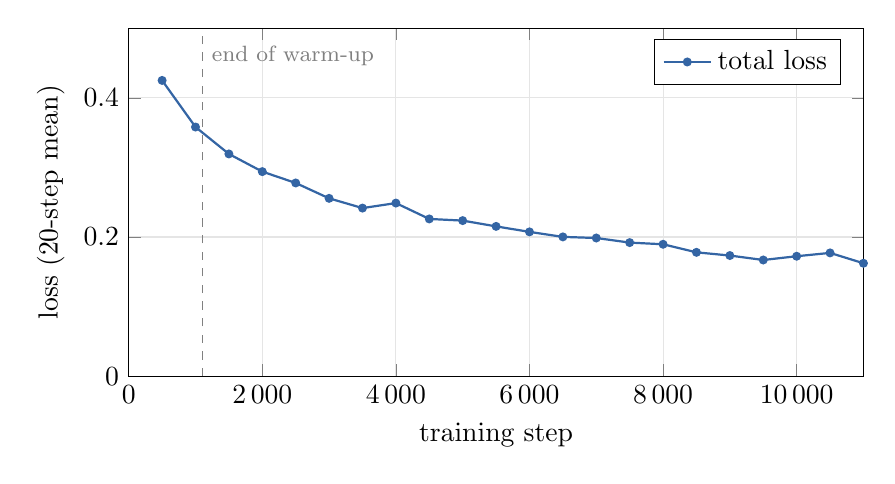
\begin{tikzpicture}
\begin{axis}[width=0.9\linewidth,height=6cm,xlabel={training step},ylabel={loss (20-step mean)},
  xmin=0,xmax=11000,ymin=0,ymax=0.5,grid=both,grid style={gray!20},legend pos=north east,
  scaled x ticks=false,xticklabel style={/pgf/number format/.cd,1000 sep={\,}}]
\addplot[thick,color=titleblue,mark=*,mark size=1.2pt] coordinates {
(500,0.4250)(1000,0.3580)(1500,0.3193)(2000,0.2939)(2500,0.2776)(3000,0.2555)(3500,0.2415)(4000,0.2487)(4500,0.2259)
(5000,0.2235)(5500,0.2152)(6000,0.2073)(6500,0.2001)(7000,0.1985)(7500,0.1919)(8000,0.1895)(8500,0.1779)(9000,0.1733)
(9500,0.1669)(10000,0.1723)(10500,0.1771)(11000,0.1622)};
\addlegendentry{total loss}
\draw[dashed,gray] (axis cs:1100,0) -- (axis cs:1100,0.5) node[pos=0.92,right,font=\footnotesize]{end of warm-up};
\end{axis}
\end{tikzpicture}
\caption{Stage 2 training loss (from \file{logs/s2_turbo.log}; step 1 loss was 2.13, off the chart). The LID-CTC term fell from 2.04
at step 1 to about 0.003 by step 1{,}000 and 0.001 at the end: the head learns quickly, and afterwards almost all of the loss is
transcription.}
\end{figure}

\begin{figure}[h]
\centering
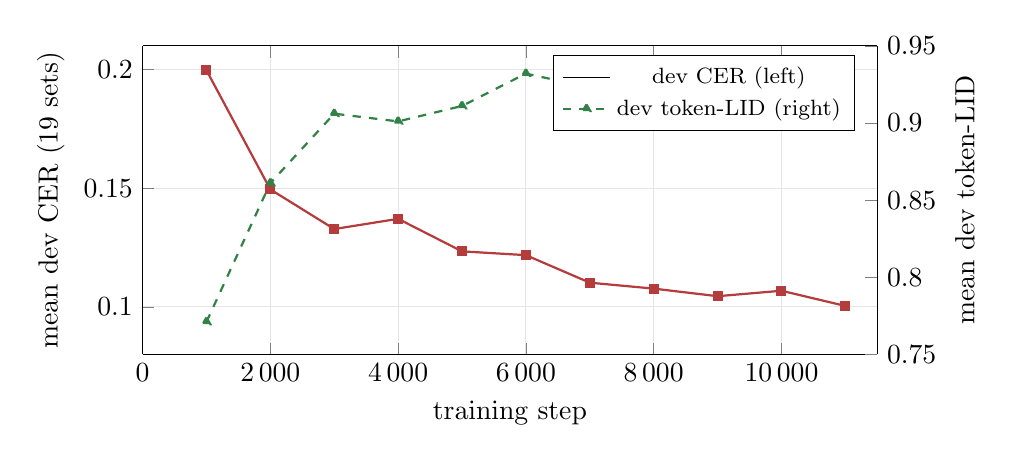
\begin{tikzpicture}
\begin{axis}[width=0.9\linewidth,height=5.5cm,xlabel={training step},ylabel={mean dev CER (19 sets)},
  xmin=0,xmax=11500,ymin=0.08,ymax=0.21,grid=both,grid style={gray!20},axis y line*=left,
  scaled x ticks=false,xticklabel style={/pgf/number format/.cd,1000 sep={\,}}]
\addplot[thick,color=thmc,mark=square*,mark size=1.4pt] coordinates {
(1000,0.1997)(2000,0.1495)(3000,0.1328)(4000,0.1371)(5000,0.1234)(6000,0.1218)(7000,0.1102)(8000,0.1077)(9000,0.1045)(10000,0.1068)(11000,0.1004)};
\label{plot:cer}
\end{axis}
\begin{axis}[width=0.9\linewidth,height=5.5cm,xmin=0,xmax=11500,ymin=0.75,ymax=0.95,axis y line*=right,axis x line=none,
  ylabel={mean dev token-LID},legend pos=north east,legend style={font=\footnotesize}]
\addlegendimage{/pgfplots/refstyle=plot:cer}\addlegendentry{dev CER (left)}
\addplot[thick,color=exc,mark=triangle*,mark size=1.6pt,dashed] coordinates {
(1000,0.771)(2000,0.861)(3000,0.906)(4000,0.901)(5000,0.911)(6000,0.932)(7000,0.923)(8000,0.912)(9000,0.929)(10000,0.930)(11000,0.931)};
\addlegendentry{dev token-LID (right)}
\end{axis}
\end{tikzpicture}
\caption{Dev-set evaluation inside the Stage 2 run (48 utterances per set, \file{runs/s2_turbo/result.json}). CER was still falling at
the last evaluation (0.105 at step 9{,}000, 0.100 at the end), while LID plateaued around 0.93 after 6{,}000 steps.}
\end{figure}

\begin{exercise}{Learning rate at step 6050}{lrcalc}
\textit{Solution.} $s=6050\ge W=1100$: $\phi=(11000-6050)/(11000-1100)=4950/9900=0.5$. LoRA learning rate $1.5\times10^{-4}$, Odia row
$1.25\times10^{-4}$, head $5\times10^{-4}$.
\end{exercise}

\begin{vivatip}
Why only one epoch? Compute: one epoch is 16.6 h on the only GPU, and the plan was to evaluate before spending more. Note also that
the dev CER evaluated every 1{,}000 steps was still improving slowly at the end, so more training (on a reseeded mix) might help;
this is listed as future work (see the dev curve above: 0.200 at step 1{,}000, 0.100 at the end, not yet flat).
\end{vivatip}

\chapter{Evaluation Protocol, Baselines and Statistics}
\chaptermark{Evaluation and Statistics}
\label{ch:eval}

\section{The test protocol}

\begin{itemize}
\item \textbf{23 test sets}: every (corpus, language) pair in the test split: FLEURS $\times7$, IndicVoices $\times6$, Kathbath
$\times5$, Lahaja hi, LibriSpeech en, Svarah en, MUCS hi and bn.
\item \textbf{100 utterances per set}, sampled with \texttt{random.Random(0)} from the test split. The \emph{same} 2{,}300 utterances
are used for every system, which makes paired comparisons possible.
\item Greedy decoding, at most 440 new tokens, the shared normaliser, micro CER per set.
\item Summary: the plain mean of the per-set CERs, plus the worst set and the standard deviation (the ML-SUPERB 2.0 style).
\end{itemize}

\section{Baselines}

\paragraph{Vanilla Whisper large-v3-turbo.} The starting point. Odia is decoded without a language token (it has none).

\paragraph{IndicConformer-600M (AI4Bharat).} A Conformer encoder (convolution + self-attention) with a CTC head over per-language
character vocabularies, trained on large AI4Bharat corpora (the same sources as IndicVoices and Kathbath). It has no English and no
LID: the language is always given. It is decoded greedily, which for CTC is simple:

\begin{definition}{Greedy CTC decoding}{greedyctc}
Take $\hat\pi_t=\argmax_c p_t(c)$ at every frame, then output $\mathcal B(\hat\pi)$ (merge repeats, drop blanks).
\end{definition}

This is exactly what \file{ic_gpu.py} does (\texttt{unique\_consecutive}, drop id 256 = blank). The ONNX runtime had no GPU kernels
for this GPU (bug 6), so the encoder and CTC head were converted to PyTorch with \texttt{onnx2torch} (verified: 23 of 24 test
transcripts identical to the CPU ONNX path, the last differs by one trailing character from batch padding).

\paragraph{Qwen3-ASR 0.6B and 1.7B.} LLM-based ASR with built-in LID for 52 languages, but of ours it supports only Hindi and
English. On other languages it answers ``Hindi'' or an unrelated language and its CER is 0.34--1.0, so it is compared only on the
Hindi and English sets, with the language forced.

\paragraph{SpeechBrain ECAPA-TDNN (VoxLingua107).} A dedicated 107-language LID model, used closed-set over the 6 of our languages it
knows (it has no Odia class). This is the external LID baseline.

\section{Statistics: how sure are we?}

A CER computed on 100 utterances is a random quantity: another 100 utterances would give a different number. We need error bars.

\begin{definition}{Percentile bootstrap confidence interval for CER}{boot}
For a test set with per-utterance edit counts $e_i$ and reference lengths $n_i$, $i=1..K$, $\widehat{\CER}=\sum_ie_i/\sum_in_i$.
For $b=1..B$ ($B=2000$), draw $K$ indices $i^{(b)}_1..i^{(b)}_K$ uniformly \emph{with replacement} and compute
$\CER^{*(b)}=\sum_je_{i^{(b)}_j}\big/\sum_jn_{i^{(b)}_j}$. The 95\% interval is $[q_{0.025},q_{0.975}]$ of
$\{\CER^{*(b)}\}$.
\end{definition}

\begin{intuition}[: why resample utterances, not characters]
Errors inside one utterance are strongly correlated (a misrecognised word costs several characters; a loop costs hundreds). The
independent unit is the utterance, so that is what we resample. Resampling the pair $(e_i,n_i)$ together keeps the ratio structure
of CER.
\end{intuition}

\begin{definition}{Paired bootstrap test}{paired}
For two systems A and B scored on the same utterances, use the \emph{same} resampled indices for both and record
$\Delta^{*(b)}=\CER_A^{*(b)}-\CER_B^{*(b)}$. The difference is called significant at 5\% if the 95\% percentile interval of
$\Delta^*$ excludes 0.
\end{definition}

\begin{proposition}{Pairing reduces variance}{pairvar}
$\mathrm{Var}(\hat C_A-\hat C_B)=\mathrm{Var}(\hat C_A)+\mathrm{Var}(\hat C_B)-2\,\mathrm{Cov}(\hat C_A,\hat C_B)$. When both systems
find the same utterances hard (positive covariance), the paired variance is smaller than for independent samples.
\end{proposition}
\begin{proof}
Bilinearity of covariance.
\end{proof}

Hard utterances (noisy, fast, rare words) are hard for every system, so the covariance is large and the paired test detects
differences that two separate CIs would not.

\begin{example}{Reading the numbers}{readci}
With 100 utterances a single cell has roughly $\pm0.01$--$0.03$ CER uncertainty. IndicConformer minus Stage 2 on FLEURS Telugu:
$+0.001$, paired 95\% interval $[-0.015,+0.016]$, which contains 0: ``not significantly different''. On IndicVoices Assamese:
$-0.110$, interval $[-0.136,-0.088]$: IndicConformer is significantly better. FLEURS Hindi is a borderline case: $-0.012$,
interval $[-0.024,-0.0002]$, which just excludes 0.
\end{example}

\begin{vivatip}[: what the bootstrap does \emph{not} cover]
It quantifies \emph{which test utterances were sampled}. It says nothing about training randomness (seed variance): only one seed was
trained, because one Stage 2 run costs 16.6 GPU hours. Say this unprompted if results are questioned.
\end{vivatip}

\section{Code-switched speech needs a different metric}
\label{sec:csmetric}

MUCS references write English words sometimes in Latin script (``computer'') and sometimes in Devanagari (\deva{कंप्यूटर}); models
also choose either. Plain CER counts ``computer'' vs \deva{कंप्यूटर} as entirely wrong, although both are correct transcriptions.

\begin{definition}{Transliteration-tolerant scores \file{cs_metric.py}}{rcer}
\textbf{rom}: normalise, then romanise \emph{every} Indic script with ISO 15919 (a hypothesis may be in another script), map anusvara
to $n$ ($m$ before $p/b$), strip diacritics, lower-case, drop a word-final inherent $a$.
\textbf{skel}: per word, keep the first letter and drop later vowels and $h,y,w$; fold $c/q/x/z/ph$; collapse repeated letters.
\[
\text{rCER}=\CER(\text{rom}(\bm r),\text{rom}(\bm h)),\qquad \text{sWER}=\WER(\text{skel}(\bm r),\text{skel}(\bm h)).
\]
\end{definition}

\begin{example}{Two spellings of the same words}{rom}
\deva{कंप्यूटर साइंस} $\xrightarrow{\text{rom}}$ ``kampyutar sains'', while ``computer science'' stays ``computer science''.
Under rom the two still differ in several letters (partial credit in rCER), but their skeletons are \emph{identical}: both
become ``kmptr sns'', so sWER counts no error. (Output of \texttt{python cs\_metric.py}.)
\end{example}

These scores are loose (partial credit for phonetically close spellings) and are applied identically to every system, so they are
suitable for \emph{ranking} systems on code-switched speech, not as absolute accuracies.

\begin{incode}
\file{analysis.py} reads the per-utterance hypotheses (\file{reports/hyps/*.jsonl}, written by every evaluation script with
\texttt{--hyps}) and produces \file{reports/analysis.md}: bootstrap CIs, paired tests vs Stage 2, rCER/sWER on MUCS, the ML-SUPERB
summary and the $7\times7$ LID confusion matrices. It regenerates byte-identically from the stored hypotheses.
\end{incode}

\chapter{Results}
\chaptermark{Results}
\label{ch:results}

All numbers: held-out test split, 100 utterances per set, the same utterances for every system (Chapter~\ref{ch:eval}).
Sources: \file{reports/experiments.md}, \file{reports/analysis.md} and\\ \file{reports/baselines/summary.md}.

\section{Speech recognition: the full table}

``Oracle'' = true language token forced; ``pred.'' = the model's own LID decides. ``+fixes'' = the two decode-time fixes of
Chapter~\ref{ch:svarah} (they change only English decoding and the LID decision).

\begin{center}
\small
\begin{tabular}{lcccccc}
\toprule
 & \multicolumn{2}{c}{Baselines (CER)} & \multicolumn{3}{c}{Stage 2 (CER)} & \\
\cmidrule(lr){2-3}\cmidrule(lr){4-6}
Set & vanilla turbo & IndicConformer & oracle & pred. & +fixes, pred. & token-LID\\
\midrule
FLEURS as & 1.204 & 0.063 & 0.084 & 0.085 & 0.084 & 0.98\\
FLEURS bn & 0.482 & 0.078 & 0.094 & 0.094 & 0.094 & 1.00\\
FLEURS hi & 0.127 & 0.065 & 0.077 & 0.077 & 0.077 & 1.00\\
FLEURS mr & 0.251 & 0.063 & 0.075 & 0.080 & 0.080 & 0.99\\
FLEURS or & 1.023 & 0.065 & 0.145 & 0.145 & 0.145 & 1.00\\
FLEURS te & 0.489 & 0.087 & 0.086 & 0.086 & 0.086 & 1.00\\
FLEURS en & 0.036 & -- & 0.042 & 0.042 & 0.042 & 1.00\\
\midrule
IndicVoices as & 2.601 & 0.055 & 0.164 & 0.224 & 0.186 & 0.66\\
IndicVoices bn & 1.185 & 0.061 & 0.119 & 0.159 & 0.143 & 0.77\\
IndicVoices hi & 0.321 & 0.068 & 0.107 & 0.119 & 0.120 & 0.81\\
IndicVoices mr & 0.716 & 0.060 & 0.124 & 0.140 & 0.140 & 0.85\\
IndicVoices or & 2.046 & 0.104 & 0.196 & 0.223 & 0.223 & 0.75\\
IndicVoices te & 1.116 & 0.081 & 0.203 & 0.209 & 0.209 & 0.95\\
\midrule
Kathbath bn & 0.505 & 0.021 & 0.044 & 0.052 & 0.052 & 0.99\\
Kathbath hi & 0.116 & 0.029 & 0.055 & 0.061 & 0.061 & 0.99\\
Kathbath mr & 0.240 & 0.029 & 0.065 & 0.066 & 0.066 & 0.99\\
Kathbath or & 1.299 & 0.026 & 0.041 & 0.041 & 0.041 & 1.00\\
Kathbath te & 0.371 & 0.037 & 0.060 & 0.060 & 0.060 & 1.00\\
\midrule
Lahaja hi & 0.259 & 0.038 & 0.064 & 0.152 & 0.147 & 0.77\\
LibriSpeech en & 0.014 & -- & 0.008 & 0.008 & 0.008 & 1.00\\
Svarah en & \textbf{0.032} & -- & 0.227 & 0.737 & 0.311 & 0.13\\
MUCS hi--en & 0.512 & 0.545 & \textbf{0.306} & 0.306 & 0.306 & 1.00\\
MUCS bn--en & 1.053 & 0.501 & \textbf{0.213} & 0.213 & 0.213 & 1.00\\
\midrule
\textbf{Mean (23 sets)} & 0.696 & (0.104 over 20) & \textbf{0.113} & 0.147 & \textbf{0.126} & \\
\bottomrule
\end{tabular}
\end{center}

\begin{figure}[h]
\centering
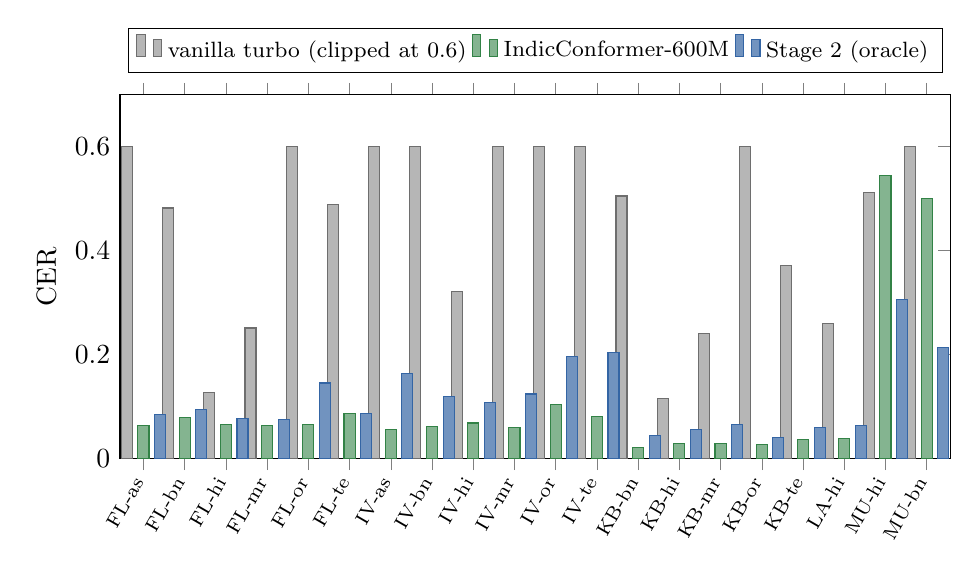
\begin{tikzpicture}
\begin{axis}[ybar,width=\linewidth,height=6.2cm,bar width=4pt,ymin=0,ymax=0.7,ytick={0,0.2,0.4,0.6},ylabel={CER},
  symbolic x coords={FL-as,FL-bn,FL-hi,FL-mr,FL-or,FL-te,IV-as,IV-bn,IV-hi,IV-mr,IV-or,IV-te,KB-bn,KB-hi,KB-mr,KB-or,KB-te,LA-hi,MU-hi,MU-bn},
  xtick=data,x tick label style={rotate=60,anchor=east,font=\scriptsize},legend style={at={(0.5,1.06)},anchor=south,legend columns=3,font=\footnotesize},
  enlarge x limits=0.03,restrict y to domain*=0:0.6]
\addplot[fill=codec!50,draw=codec] coordinates {(FL-as,0.6)(FL-bn,0.482)(FL-hi,0.127)(FL-mr,0.251)(FL-or,0.6)(FL-te,0.489)(IV-as,0.6)(IV-bn,0.6)(IV-hi,0.321)(IV-mr,0.6)(IV-or,0.6)(IV-te,0.6)(KB-bn,0.505)(KB-hi,0.116)(KB-mr,0.240)(KB-or,0.6)(KB-te,0.371)(LA-hi,0.259)(MU-hi,0.512)(MU-bn,0.6)};
\addplot[fill=exc!60,draw=exc] coordinates {(FL-as,0.063)(FL-bn,0.078)(FL-hi,0.065)(FL-mr,0.063)(FL-or,0.065)(FL-te,0.087)(IV-as,0.055)(IV-bn,0.061)(IV-hi,0.068)(IV-mr,0.060)(IV-or,0.104)(IV-te,0.081)(KB-bn,0.021)(KB-hi,0.029)(KB-mr,0.029)(KB-or,0.026)(KB-te,0.037)(LA-hi,0.038)(MU-hi,0.545)(MU-bn,0.501)};
\addplot[fill=titleblue!70,draw=titleblue] coordinates {(FL-as,0.084)(FL-bn,0.094)(FL-hi,0.077)(FL-mr,0.075)(FL-or,0.145)(FL-te,0.086)(IV-as,0.164)(IV-bn,0.119)(IV-hi,0.107)(IV-mr,0.124)(IV-or,0.196)(IV-te,0.203)(KB-bn,0.044)(KB-hi,0.055)(KB-mr,0.065)(KB-or,0.041)(KB-te,0.060)(LA-hi,0.064)(MU-hi,0.306)(MU-bn,0.213)};
\legend{vanilla turbo (clipped at 0.6),IndicConformer-600M,Stage 2 (oracle)}
\end{axis}
\end{tikzpicture}
\caption{Indic and code-switched test sets. Grey bars at 0.6 are clipped; the true values are above 1 (repetition loops).}
\end{figure}

\subsection*{What the table says}
\begin{enumerate}
\item \textbf{Fine-tuning turns an unusable model into a usable one} on every Indic set: mean CER 0.696 $\to$ 0.113. Every vanilla
CER above 1 was a loop.
\item \textbf{Odia works} through the new token (Kathbath 0.041, FLEURS 0.145). FLEURS Odia is the weakest FLEURS language; it has
the least FLEURS training data (3.4 h).
\item \textbf{English is preserved} on read speech (LibriSpeech 0.014 $\to$ 0.008; FLEURS 0.036 $\to$ 0.042) but \textbf{broken on
Indian-accented English} (Svarah 0.032 $\to$ 0.227). Chapter~\ref{ch:svarah} is devoted to this.
\item \textbf{IndicConformer is better on monolingual in-domain sets.} The paired bootstrap interval excludes 0 on 17 of the 18
monolingual Indic sets (all except FLEURS Telugu; FLEURS Hindi only just). The gap is largest on IndicVoices (0.04--0.12). Two caveats:
IndicConformer was trained on far more AI4Bharat data from the \emph{same sources} as IndicVoices and Kathbath, and it has no
English, no LID and no code-switch ability. On FLEURS, which is out of domain for both, the gap is small (0.01--0.02 except Odia).
\item \textbf{Code-switching: Stage 2 is clearly best} (MUCS hi 0.306 vs 0.545, bn 0.213 vs 0.501), significant in the paired test.
\end{enumerate}

\section{The cost of LID errors}

Mean CER: oracle 0.113, predicted 0.147, predicted with the calibrated rule 0.126. Without Svarah the routing cost is small almost
everywhere; it is large exactly where LID is weak:

\begin{center}
\begin{tabular}{lccc}
\toprule
Set & oracle & predicted (+fixes) & gap\\
\midrule
Lahaja hi & 0.064 & 0.147 & $+0.083$\\
IndicVoices as & 0.164 & 0.186 & $+0.022$\\
IndicVoices bn & 0.119 & 0.143 & $+0.024$\\
Svarah en & 0.227 (0.114 ASCII) & 0.311 & $+0.197$\\
\bottomrule
\end{tabular}
\end{center}

\section{Language identification}

Pooled recall over all test sets (rows: true language):

\begin{center}
\small
\begin{tabular}{lccccc}
\toprule
Language & vanilla token & ECAPA (closed set) & Stage 2 token & Stage 2 head & Stage 2 calibrated\\
\midrule
hi & 0.84 & 0.90 & 0.91 & 0.91 & 0.91\\
en & 1.00 & 0.71 & 0.71 & 0.75 & \textbf{0.84}\\
te & 0.14 & 0.97 & 0.98 & 0.98 & 0.98\\
as & 0.00 & 0.92 & 0.82 & 0.92 & 0.89\\
or & no token & no class & 0.92 & 0.90 & 0.92\\
bn & 0.42 & 0.81 & 0.94 & 0.94 & 0.94\\
mr & 0.52 & 0.89 & 0.94 & 0.93 & 0.94\\
\bottomrule
\end{tabular}
\end{center}

Confusion matrix of the Stage 2 decoder token (counts; rows true, columns predicted):

\begin{center}
\begin{tabular}{l|ccccccc|c}
 & hi & en & te & as & or & bn & mr & recall\\\hline
hi & \textbf{457} & $\cdot$ & 7 & 1 & 17 & 3 & 15 & 0.91\\
en & 26 & \textbf{213} & 21 & 1 & 15 & 16 & 8 & 0.71\\
te & $\cdot$ & $\cdot$ & \textbf{295} & $\cdot$ & 4 & $\cdot$ & 1 & 0.98\\
as & 3 & $\cdot$ & 4 & \textbf{164} & 22 & 7 & $\cdot$ & 0.82\\
or & 9 & $\cdot$ & 8 & $\cdot$ & \textbf{275} & 1 & 7 & 0.92\\
bn & 5 & $\cdot$ & 5 & $\cdot$ & 11 & \textbf{376} & 3 & 0.94\\
mr & 3 & $\cdot$ & 3 & $\cdot$ & 5 & 6 & \textbf{283} & 0.94\\
\end{tabular}
\end{center}

\begin{itemize}
\item FLEURS, Kathbath, LibriSpeech and MUCS sets are at 0.98--1.00. Errors concentrate in spontaneous IndicVoices (0.66--0.95),
Lahaja (0.77) and Svarah.
\item \textbf{Excluding Svarah, English recall is 1.00} (200/200). All 87 English errors are Indian-accented English, spread over
every Indic language.
\item The \tok{or} column absorbs errors (17 hi, 22 as, 15 en, 11 bn), as discussed in Chapter~\ref{ch:odia}.
\item The LID head helps most on Assamese (0.82 $\to$ 0.92); the calibrated rule combines both opinions plus an English bias.
\item Against the dedicated ECAPA LID model, Stage 2 is equal or better on every Indic language and also covers Odia. ECAPA fails on
Indian English in exactly the same way (Svarah 0.14), which suggests the difficulty is intrinsic to accented English, not to our
model alone.
\end{itemize}

\section{Robustness}

\paragraph{Hallucination} (Stage 2, 100 held-out noise/music clips per language): 0.01, 0.00, 0.01, 0.01, 0.01, 0.01, 0.01 for
hi, en, te, as, or, bn, mr; mean output tokens on noise 0--1.5; false silence on real speech 0.00 in all languages. Vanilla: about
1.0.

\begin{figure}[h]
\centering
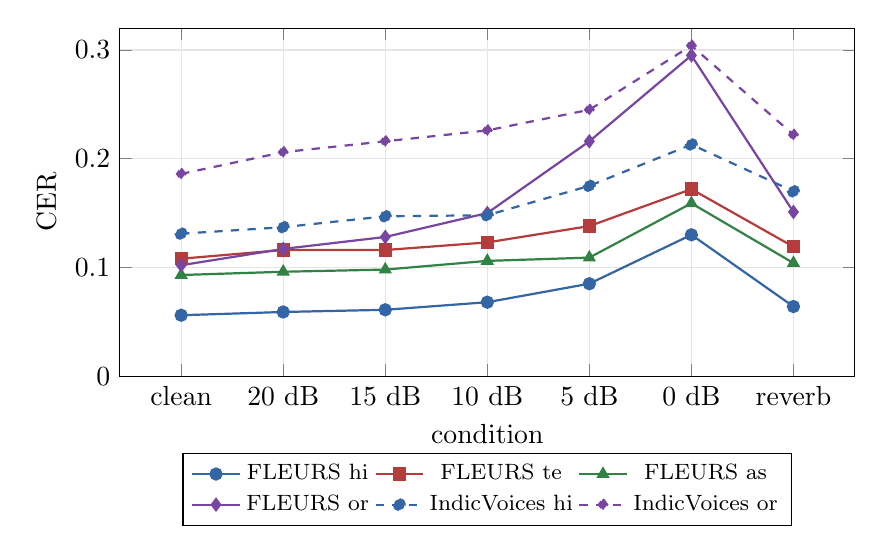
\begin{tikzpicture}
\begin{axis}[width=0.9\linewidth,height=6cm,xlabel={condition},ylabel={CER},
  symbolic x coords={clean,20 dB,15 dB,10 dB,5 dB,0 dB,reverb},xtick=data,ymin=0,ymax=0.32,grid=major,grid style={gray!20},
  legend style={at={(0.5,-0.22)},anchor=north,font=\footnotesize},legend columns=3]
\addplot[thick,mark=*,color=titleblue] coordinates {(clean,0.056)(20 dB,0.059)(15 dB,0.061)(10 dB,0.068)(5 dB,0.085)(0 dB,0.130)(reverb,0.064)};
\addplot[thick,mark=square*,color=thmc] coordinates {(clean,0.108)(20 dB,0.116)(15 dB,0.116)(10 dB,0.123)(5 dB,0.138)(0 dB,0.172)(reverb,0.119)};
\addplot[thick,mark=triangle*,color=exc] coordinates {(clean,0.093)(20 dB,0.096)(15 dB,0.098)(10 dB,0.106)(5 dB,0.109)(0 dB,0.159)(reverb,0.104)};
\addplot[thick,mark=diamond*,color=hwc] coordinates {(clean,0.102)(20 dB,0.117)(15 dB,0.128)(10 dB,0.150)(5 dB,0.216)(0 dB,0.295)(reverb,0.151)};
\addplot[thick,dashed,mark=*,color=titleblue] coordinates {(clean,0.131)(20 dB,0.137)(15 dB,0.147)(10 dB,0.148)(5 dB,0.175)(0 dB,0.213)(reverb,0.170)};
\addplot[thick,dashed,mark=diamond*,color=hwc] coordinates {(clean,0.186)(20 dB,0.206)(15 dB,0.216)(10 dB,0.226)(5 dB,0.245)(0 dB,0.304)(reverb,0.222)};
\legend{FLEURS hi,FLEURS te,FLEURS as,FLEURS or,IndicVoices hi,IndicVoices or}
\end{axis}
\end{tikzpicture}
\caption{Stage 2 under held-out noise (60 utterances per set, \file{reports/snr_s2_turbo.json}). Degradation is gradual; Odia is the
most noise-sensitive. Compare vanilla Whisper-small on FLEURS hi: 0.357 clean, 0.806 at 0 dB.}
\end{figure}

\section{Code-switching with the tolerant metrics}

\begin{center}
\begin{tabular}{llccc}
\toprule
System & set & CER & rCER & sWER\\
\midrule
Stage 2 & MUCS hi & \textbf{0.306} & \textbf{0.251} & \textbf{0.294}\\
IndicConformer & MUCS hi & 0.545 & 0.367 & 0.387\\
vanilla turbo & MUCS hi & 0.512 & 0.366 & 0.409\\
Qwen3-ASR-1.7B & MUCS hi & 0.482 & 0.306 & 0.316\\
Qwen3-ASR-0.6B & MUCS hi & 0.417 & 0.307 & 0.356\\
\midrule
Stage 2 & MUCS bn & \textbf{0.213} & \textbf{0.173} & \textbf{0.254}\\
IndicConformer & MUCS bn & 0.501 & 0.326 & 0.439\\
vanilla turbo & MUCS bn & 1.053 & 0.749 & 1.382\\
\bottomrule
\end{tabular}
\end{center}
The ranking survives the script-tolerant metrics, so Stage 2's advantage is not an artefact of choosing the same script as the
references.

\section{Against Qwen3-ASR on Hindi and English}

\begin{center}
\begin{tabular}{lcccc}
\toprule
Set & Qwen3-0.6B & Qwen3-1.7B & Stage 2 oracle & Stage 2 +fixes pred.\\
\midrule
FLEURS hi & 0.107 & 0.068 & 0.077 & 0.077\\
IndicVoices hi & 0.144 & 0.100 & 0.107 & 0.120\\
Kathbath hi & 0.077 & \textbf{0.044} & 0.055 & 0.061\\
Lahaja hi & 0.118 & 0.076 & 0.064 & 0.147\\
MUCS hi--en & 0.417 & 0.482 & \textbf{0.306} & 0.306\\
FLEURS en & 0.036 & \textbf{0.027} & 0.042 & 0.042\\
LibriSpeech en & 0.008 & 0.006 & 0.008 & 0.008\\
Svarah en & 0.134 & \textbf{0.101} & 0.227 (0.114 ASCII) & 0.311\\
\bottomrule
\end{tabular}
\end{center}
Paired tests vs Stage 2 (oracle): Qwen3-1.7B is significantly better on Kathbath hi, FLEURS en and Svarah; not significantly
different on FLEURS hi, IndicVoices hi and Lahaja; significantly worse on MUCS hi. Stage 2 is significantly better than Qwen3-0.6B
on all Hindi sets. A 1.7B model trained for Hindi and English is level with our 7-language model on monolingual Hindi and clearly
behind on code-switching.

\section{Summary in the ML-SUPERB style}

\begin{center}
\begin{tabular}{lcccc}
\toprule
System & sets & mean CER & worst set & std\\
\midrule
Stage 2 (oracle) & 23 & 0.113 & MUCS hi 0.306 & 0.072\\
Stage 2 + fixes (pred.) & 23 & 0.126 & Svarah 0.311 & 0.081\\
Stage 2 (pred., no fixes) & 23 & 0.147 & Svarah 0.737 & 0.145\\
vanilla turbo & 23 & 0.696 & IndicVoices as 2.601 & 0.650\\
IndicConformer & 20 & 0.104 & MUCS hi 0.545 & 0.142\\
\bottomrule
\end{tabular}
\end{center}

\begin{vivatip}[: the one-sentence summary]
``One 809 M-parameter Whisper with 20 M trained LoRA parameters, a new Odia token and an encoder LID head transcribes seven
languages at a mean CER of 0.113 (0.126 with its own LID), almost never hallucinates on noise, beats every baseline on code-switched
speech, trails the in-domain Indic specialist on monolingual Indic speech, and regressed on Indian-accented English.''
\end{vivatip}

\chapter{The Indian-English Regression and Two Decode-Time Fixes}
\chaptermark{The Indian-English Regression}
\label{ch:svarah}

\section{The symptom}

Svarah is Indian-accented English (117 speakers from 65 districts). Vanilla turbo transcribes it at CER 0.032 and identifies it as
English 99\% of the time. After fine-tuning:
\begin{itemize}
\item token LID 0.13 (head 0.25): Svarah is now mostly called Hindi, Telugu, Bengali, Odia\dots;
\item even with \tok{en} forced (oracle), CER 0.227; with predicted LID, 0.737.
\end{itemize}

\section{Diagnosis from the per-utterance hypotheses}

\begin{center}
\begin{tabular}{lccc}
\toprule
Subset of the 100 Svarah test utterances (oracle \tok{en}) & $n$ & Stage 2 CER & vanilla CER\\
\midrule
hypothesis contains non-Latin script & 39 & 0.715 & 0.059\\
reference contains digits & 12 & 0.585 & 0.040\\
rest & 55 & 0.048 & 0.023\\
\bottomrule
\end{tabular}
\end{center}
(6 utterances are in both of the first two rows.)

Two mechanisms:
\begin{enumerate}
\item \textbf{Script leakage.} In 39\% of utterances, even when told ``English'', the model writes English words in Bengali, Telugu or
Devanagari script. The training mix contains no Indian-accented English: the only English is LibriSpeech (American/British audiobooks)
and FLEURS. Indian-accented English is acoustically closer to the Indic training data (and to the English words inside MUCS, which
are often written in Indic script) than to LibriSpeech, so the model maps it to Indic outputs.
\item \textbf{Number style.} References use digits (``25''); the model, like LibriSpeech, spells numbers out (``twenty five''). The
normaliser does not verbalise digits (Chapter~\ref{ch:metrics}), so this counts as errors.
\end{enumerate}

\begin{intuition}[: catastrophic forgetting, in its classic form]
Vanilla Whisper handled Indian English well because its 680{,}000-hour pretraining included it. Our fine-tuning distribution
contained none, and nothing in the objective rewarded keeping that ability. Fine-tuning optimises the training mixture; abilities
outside it are free to drift.
\end{intuition}

\section{Fix 1: ASCII-only English decoding}

\begin{definition}{Logit masking}{mask}
Let $\mathcal A\subset\{1..V\}$ be the tokens whose decoded string is pure ASCII. When decoding with \tok{en}, set $z_{t,v}=-\infty$ for
$v\notin\mathcal A$ at every step. Then
\[
\tilde p(v\mid\cdot)=\frac{e^{z_v}\1[v\in\mathcal A]}{\sum_{u\in\mathcal A}e^{z_u}}=p(v\mid\cdot,\ v\in\mathcal A),
\]
the model's distribution \emph{conditioned} on producing an ASCII token.
\end{definition}

11{,}707 vocabulary tokens are not pure ASCII. The effect is surgical: Svarah oracle CER $0.227\to\mathbf{0.114}$, and no other English
or MUCS set changes (MUCS is decoded with \tok{hi}/\tok{bn}, not \tok{en}).

\section{Fix 2: a calibrated LID rule}

Fix 1 only helps if \tok{en} is chosen. The second fix improves the decision itself by combining three pieces of evidence.

\begin{definition}{Calibrated LID score}{rule}
For each $\ell\in\mathcal L$,
\[
\mathrm{score}(\ell)=\log\hat p_{\text{tok}}(\ell\mid\vx)+b\cdot\1[\ell=\text{en}]+w\cdot\log q(\ell\mid\vx),\qquad
\hat\ell=\argmax_\ell\mathrm{score}(\ell),
\]
where $\hat p_{\text{tok}}$ is the closed-set token probability (Definition~\ref{def:tokenlid}) and $q$ the normalised head mass
(Chapter~\ref{ch:ctc}, clamped at $10^{-6}$).
\end{definition}

\begin{proposition}{The rule is a weighted product of experts}{poe}
$\hat\ell=\argmax_\ell\ \hat p_{\text{tok}}(\ell)\,q(\ell)^{w}\,e^{b\1[\ell=\text{en}]}$, i.e.\ the argmax of the normalised
distribution $\pi(\ell)\propto\hat p_{\text{tok}}(\ell)\,q(\ell)^w\,e^{b\1[\ell=\text{en}]}$.
\end{proposition}
\begin{proof}
$\exp$ is increasing, so $\argmax$ of the score equals $\argmax$ of its exponential, which is the product. Normalising by a positive
constant does not change the argmax.
\end{proof}

$w$ sets how much the encoder head is trusted relative to the decoder token; $b$ is a prior log-odds shift toward English.

\paragraph{Fitting.} A grid $w\in\{0,0.25,0.5,1,2\}$, $b\in\{0,0.25,\dots,30\}$ (605 points). Objective: \emph{macro} LID accuracy over
the calibration sets, ties broken toward the smallest change ($-|b|-w$). Calibration data: the dev split (100 per set) plus a
\textbf{speaker-disjoint Svarah calibration set}: Svarah has no speaker ids, so a speaker is approximated by the demographic profile
(gender, age group, native state and district, qualification, occupation; 115 profiles). All profiles occurring in the 100 scored test
utterances are excluded; 300 utterances from 54 remaining profiles are used. The test split is never used for fitting.

\paragraph{Result.} $b=22.25$, $w=2.0$; calibration macro LID $0.900\to0.919$.

\begin{example}{What $b=22.25$ means}{bmeaning}
In probability terms the English prior is multiplied by $e^{22.25}\approx4.6\times10^{9}$. That sounds absurd, but the grid search
kept gaining calibration accuracy as $b$ grew to this size. An utterance flips to English only if its score gap
$\mathrm{score}(\ell_{\text{win}})-\mathrm{score}(\text{en})$ without the bias is below $b$, so many Svarah utterances must have had
gaps of the order of 20 nats: the fine-tuned token is extremely over-confident. Yet on genuine Indic speech the gap in favour of the
true language is evidently even larger, because the same shift almost never flips a correct answer: on test no set loses more than
0.02 LID accuracy.
\end{example}

\begin{center}
\begin{tabular}{lcccc}
\toprule
Test set & LID before & LID after & pred.\ CER before & pred.\ CER after\\
\midrule
Svarah en & 0.13 & 0.51 & 0.737 & 0.311\\
IndicVoices as & 0.66 & 0.77 & 0.224 & 0.186\\
IndicVoices bn & 0.77 & 0.78 & 0.159 & 0.143\\
Lahaja hi & 0.77 & 0.78 & 0.152 & 0.147\\
\bottomrule
\end{tabular}
\end{center}
Mean predicted-LID CER over 23 sets: $0.147\to0.126$.

\begin{vivatip}[: honest caveats about the calibration]
(1) $w=2.0$ is the edge of the grid; but the macro gain from $w=0.5$ to $2$ is only 0.003, so extending the grid would change little.
(2) The calibration Svarah utterances come from the Svarah corpus itself (different speakers, same recording conditions), so the
fix is tuned to this kind of accent and microphone. (3) Speakers are approximated by profile; two people with the same profile would
be merged (conservative for disjointness).
\end{vivatip}

\section{What would fix it properly}

Svarah is still far behind vanilla (0.311 vs 0.032). The decode-time fixes treat the symptom. A real fix changes training:
\begin{itemize}
\item add Indian-accented English to the mix (Svarah-like data, NPTEL lecture audio);
\item or a \emph{rehearsal / distillation} term that keeps the fine-tuned model's English outputs close to the vanilla model's, e.g.\
add $\beta\,\mathrm{KL}\big(p_{\text{vanilla}}(\cdot\mid\vx)\,\|\,p_\theta(\cdot\mid\vx)\big)$ on English audio;
\item and verbalise digits consistently in references and targets.
\end{itemize}
Each needs a retraining run of about a day.

\begin{incode}
\file{eval_whisper.py --en_ascii --lid_rule runs/s2_turbo/lid_rule.json}; \file{make_svarah_calib.py} builds the calibration set;
\file{lid_calib.py} fits $(b,w)$ and writes \file{lid_rule.json}. The demo uses both fixes.
\end{incode}

\begin{exercise}{Why must the Svarah calibration utterances be speaker-disjoint from the scored ones?}{calibdisj}
\textit{Solution.} $b$ is fitted to maximise accuracy on the calibration set. If the scored test speakers were in it, $b$ could be
tuned to those speakers' voices and the reported test improvement (0.13 $\to$ 0.51) would be optimistic: the same test-set
contamination that speaker-disjoint splits prevent in training (Chapter~\ref{ch:data}).
\end{exercise}

\chapter{The Demo: Long Audio, VAD Chunking and One Language Decision}
\chaptermark{The Demo}
\label{ch:demo}

\section{What the demo does}

\file{src/demo.py} is a Gradio web app: upload or record audio; it shows the detected language with closed-set confidences, the
encoder head's opinion, and the transcript. The language can also be forced from a drop-down.

\section{Why the audio must be cut}

The model was trained on single utterances of at most 30 s and at most 440 text tokens. Real recordings are longer. The first
version simply cut fixed 30-s windows. Two failures were observed:
\begin{enumerate}
\item On a packed 30-s window of a 51-s clip the model \emph{skipped a whole sentence}, and the LID head's posteriors became nearly
uniform (it had only seen single utterances).
\item 25-s Telugu chunks overflowed the 440-token budget (Telugu costs up to about 45 tokens per second; Exercise~\ref{exr:ex27}).
\end{enumerate}

\section{VAD-based chunking}

\begin{definition}{Voice activity detection (VAD)}{vad}
A VAD model labels short frames as speech or non-speech. Silero VAD (a small neural network) returns speech segments
$[s_1,e_1],[s_2,e_2],\dots$ in samples (minimum pause here: 200 ms).
\end{definition}

\begin{definition}{The chunking rule}{chunk}
Let $L_{\max}=12\,\text{s}\cdot16000$. If the clip is at most $L_{\max}$, keep it whole. Otherwise the candidate cut points are the
midpoints of the pauses, $c_k=\lfloor(e_k+s_{k+1})/2\rfloor$. Starting at $0$, repeatedly cut at the \emph{last} candidate within
$L_{\max}$ of the current start (greedy packing); if none exists (a single stretch of speech longer than 12 s), cut hard at
$L_{\max}$. Chunks shorter than 0.3 s are dropped unless nothing else is left.
\end{definition}

Cutting in pauses keeps words intact; greedy packing makes chunks as long as allowed, which gives the decoder more context. No audio
is discarded.

\section{One language for the whole clip}

Each chunk $c$ gives a score vector $\mathrm{score}_c(\ell)$ (token log-probability plus the calibrated rule terms of
Chapter~\ref{ch:svarah}). The clip's language is
\[
\hat\ell=\argmax_\ell\sum_c\mathrm{score}_c(\ell),
\]
and the displayed confidence is $\softmax_\ell\big(\sum_c\mathrm{score}_c(\ell)\big)$.

\begin{proposition}{Summing log-scores is naive-Bayes pooling}{nb}
If chunks were conditionally independent given the language and each $\mathrm{score}_c$ were a log-likelihood, then
$\sum_c\mathrm{score}_c(\ell)=\log\prod_cp(\text{chunk}_c\mid\ell)$, the log-likelihood of the whole clip, and its argmax is the
maximum-likelihood language.
\end{proposition}
\begin{proof}
Independence turns the joint likelihood into a product; $\log$ turns the product into a sum.
\end{proof}
In practice chunks are not independent (same speaker, same channel), so the pooled confidence is over-confident for long clips; the
argmax is still a sensible decision.

All chunks are then decoded with the chosen language (ASCII-only if English), and the transcripts are joined with spaces.

\section{Measured quality}

On 50--70 s concatenations of FLEURS utterances the chunked demo gives CER 0.05 (Assamese), 0.15 (Hindi) and 0.18 (Telugu).

\begin{vivatip}[: bug fixed in the fourth review]
Gradio delivers integer PCM. The first version detected ``integer audio'' by checking $\max|x|>1$ \emph{after} casting to float:
silent int16 audio was not rescaled, and int32 audio was divided by 32768 instead of $2^{31}$. It now checks the dtype and divides by
\texttt{np.iinfo(dtype).max+1}.
\end{vivatip}

\chapter{Bugs, Lessons, Limitations and Future Work}
\chaptermark{Lessons and Limitations}
\label{ch:lessons}

\section{The bugs that would have changed conclusions}

The project log records 26 bugs. Most were cosmetic or caught before they mattered. These would have changed reported numbers or
decisions:

\begin{center}
\small
\begin{tabularx}{\linewidth}{lYY}
\toprule
\# & What was wrong & What it would have done\\
\midrule
4 & Official IndicVoices/Kathbath ``valid'' sets share 1{,}217 / 40 speakers with ``train'' & optimistic test numbers (test speakers seen in training)\\
5 & Baseline decoding capped at 200 new tokens; Indic references reach 650 tokens & truncated outputs, wrong baseline CER\\
9 & LID-CTC loss not normalised by frames ($\approx$300 at start) & auxiliary loss would swamp the ASR loss\\
10 & \texttt{begin\_suppress\_tokens} forbids EOT first, so empty output impossible & hallucination stuck near 100\%; led to a wrong diagnosis and an unnecessary 30$\times$ loss weight\\
11 & 92 ``RIRs'' were noise recordings; multi-mic averaging & reverb augmentation and reverb test partly noise\\
12 & speed perturbation stretched clips past 30 s while labels stayed full & taught the model to hallucinate cut-off words\\
13 & random language label on non-speech clips was a target & label noise in both LID outputs\\
15 & \texttt{convert\_tokens\_to\_ids("<|or|>")} returns EOT silently & Odia evaluation prompted with EOT\\
\bottomrule
\end{tabularx}
\end{center}

\section{Lessons}

\begin{enumerate}
\item \textbf{Verify the measurement before the model.} A metric that does not move at all (bug 10) is more often a measurement bug
than a modelling failure.
\item \textbf{Check official splits.} ``Valid'' does not mean ``speaker-disjoint''.
\item \textbf{Silent fallbacks are the dangerous ones.} An unknown token mapped to EOT, a cap of 200 tokens, a noise file in the RIR
folder: none raised an error.
\item \textbf{Test a suspicion before acting on it.} The emb-lr sweep showed that the suspected cause of an all-Odia transient was
wrong (Chapter~\ref{ch:odia}).
\item \textbf{Make every random choice a function of (seed, epoch, index).} It made resumption exact and refactoring verifiable:
after the final code cleanup, the test evaluation reproduced all 23 Stage 2 results and all IndicConformer results exactly.
\item \textbf{Fine-tuning optimises the mixture you give it.} Anything outside it (Indian English) may be forgotten.
\item \textbf{Unified memory is shared.} Three parallel Whisper-small runs filled 122 GB and all stalled at step 1; runs were made
sequential.
\end{enumerate}

\section{Limitations}

\begin{itemize}
\item $n=100$ per test set and \textbf{one training seed}: bootstrap CIs cover test sampling, not training variance.
\item One epoch of one deterministic mix; IndicVoices is sub-sampled to 0.5--0.7$\times$ per epoch.
\item IndicConformer's advantage may be partly in-domain; FLEURS (out of domain for both) shows a smaller gap.
\item MUCS references mix scripts inconsistently; rCER and sWER are loose comparison metrics, not absolute accuracies.
\item Digits vs number words are not normalised; parenthesised FLEURS text is dropped (inflates FLEURS CER by 0.005--0.02 for all
systems).
\item The robustness test noise comes from the same MUSAN categories as the training noise (held-out files only); no UrbanSound or
DEMAND test was run. MUSAN ``music'' includes some tracks with vocals, used as empty-target non-speech.
\item Not done: synthetic Hinglish via TTS, the words-per-second truncation guard (loop rate is already about 0), Voice of India and
Vistaar benchmarks (not available).
\end{itemize}

\section{Future work}

\begin{enumerate}
\item Indian-accented English in training, or a distillation term toward vanilla Whisper on English (Chapter~\ref{ch:svarah}).
\item A second epoch on a reseeded mix (\texttt{balanced\_mix.py 1}); the dev curve had not flattened.
\item Test why \tok{or} absorbs LID errors, e.g.\ by also unfreezing the other six language rows with the same mask.
\item Multiple seeds for the final configuration.
\item Fix the normaliser's parenthesis rule for FLEURS and verbalise numbers consistently.
\end{enumerate}

\chapter{Formula Sheet and Viva Practice}
\chaptermark{Formula Sheet and Viva}
\label{ch:formulas}

\section{One-page formula sheet}

\begin{tcolorbox}[colback=white,colframe=titleblue,title={Audio and Whisper}]
$x[n]=x_c(n/f_s)$, $f_s=16$ kHz $\cdot$ STFT 25 ms window, 10 ms hop $\cdot$ $\mathrm{mel}(f)=2595\log_{10}(1+f/700)$ $\cdot$
$\bm F=(\max(L,\max L-8)+4)/4$, $L=\log_{10}\max(\mathcal M,10^{-10})$ $\cdot$ input $128\times3000$ $\cdot$ encoder 1500 frames, 50/s
$\cdot$ $T=\min(1500,\lfloor50D\rfloor+1)$ $\cdot$ decoder $\le448$ positions; text $\le440$ tokens $\cdot$ Indic 17--45 tokens/s,
English $\approx3$.
\end{tcolorbox}

\begin{tcolorbox}[colback=white,colframe=titleblue,title={Metrics and statistics}]
$D[i,j]=\min\{D[i-1,j]+1,\,D[i,j-1]+1,\,D[i-1,j-1]+\1[r_i\ne h_j]\}$ $\cdot$ $\CER=\sum(S+D+I)/\sum N$ (can exceed 1) $\cdot$
$|m-n|\le d\le\max(m,n)$ $\cdot$ bootstrap: resample utterances with replacement, $B=2000$, percentile 95\% CI $\cdot$ paired:
same indices for both systems, significant if CI of $\Delta$ excludes 0 $\cdot$ routing cost $=\CER_{\text{pred}}-\CER_{\text{oracle}}$.
\end{tcolorbox}

\begin{tcolorbox}[colback=white,colframe=titleblue,title={Model and training}]
$p(\vy\mid\vx)=\prod_tp(y_t\mid\vy_{<t},\vx)$ $\cdot$ $\nabla_{\vz}(-\log\softmax(\vz)_y)=\bm p-\bm e_y$ $\cdot$
$\mathrm{Attn}=\softmax(QK^\top/\sqrt{d_k}+M)V$ $\cdot$ LoRA $W_0+\frac\alpha rBA$, $B_0=0$, $r=32$, $\alpha=64$, params $r(d_{\text{in}}+d_{\text{out}})$
$\cdot$ trained LoRA 20.48 M (22 enc + 4 dec layers) $\cdot$ \tok{or} $=$ row $51866$, init from \tok{bn}, gradient mask, wd 0 $\cdot$
$\mathcal L=\mathcal L_{\text{CE}}+0.3\,\frac{1}{|\mathcal S|}\sum_i\ell_{\text{CTC},i}/T_i$ $\cdot$ AdamW $(0.9,0.98,10^{-6})$, lr $3\times10^{-4}$
(LoRA), $2.5\times10^{-4}$ (row), $10^{-3}$ (head) $\cdot$ warm-up 10\% then linear decay $\cdot$ clip norm 1 $\cdot$ $11{,}000\times32$.
\end{tcolorbox}

\begin{tcolorbox}[colback=white,colframe=titleblue,title={CTC, data, robustness, LID rule}]
$p(\vy\mid\vx)=\sum_{\bm\pi\in\mathcal B^{-1}(\vy)}\prod_tp_t(\pi_t)$ $\cdot$ single label: $\sum_{s\le e}\prod_{t<s}p_t(\blank)\prod_{s}^{e}p_t(\ell)\prod_{t>e}p_t(\blank)$,
$T(T+1)/2$ paths $\cdot$ head decision $\argmax_\ell\sum_tp_t(\ell)$ $\cdot$ mix: $s_c=h_c\min(3,h_{\max}/h_c)$, share cap 0.7, 90 h per
language, total $7\cdot90/(1-0.1)=700$ h $\cdot$ noise gain $g=\sqrt{P_s/(P_n10^{\sigma/10})}$, $\sigma\sim\mathcal U(0,20)$ $\cdot$
speed $\pm10\%$ only if $<27$ s $\cdot$ 5\% non-speech, target EOT, language masked $\cdot$ hallucination $=$ $>5$ tokens on noise,
with \texttt{begin\_suppress\_tokens} off $\cdot$ score $=\log\hat p_{\text{tok}}+22.25\,\1[\text{en}]+2\log q$.
\end{tcolorbox}

\begin{tcolorbox}[colback=white,colframe=titleblue,title={Headline numbers (test, 23 sets $\times$ 100 utterances)}]
Mean CER: vanilla 0.696 $\to$ Stage 2 oracle \textbf{0.113}, predicted 0.147, predicted + fixes \textbf{0.126} $\cdot$
IndicConformer 0.104 over its 20 sets (significantly better on 17 of 18 monolingual Indic sets) $\cdot$ MUCS hi/bn 0.306/0.213 vs
IndicConformer 0.545/0.501 $\cdot$ hallucination $\approx1.0\to\le0.01$ $\cdot$ Svarah 0.032 (vanilla) vs 0.227 oracle, 0.114 ASCII,
0.311 predicted + fixes $\cdot$ Odia Kathbath 0.041, FLEURS 0.145 $\cdot$ 16.6 h training at 5.9 utt/s.
\end{tcolorbox}

\section{Likely viva questions, with answer sketches}

\begin{enumerate}[leftmargin=*,label=\textbf{Q\arabic*.}]
\item \textbf{Why Whisper and not IndicConformer as the base?} IndicConformer has no English, no LID and no code-switch support; the
project requires one model with integrated LID. Whisper's decoder already has a language token and a multilingual text decoder,
and turbo is fast. The price: worse in-domain monolingual Indic CER.

\item \textbf{Why does vanilla Whisper's CER exceed 1?} CER counts insertions; repetition loops make hypotheses much longer than
references (Proposition~\ref{prop:cerbound}).

\item \textbf{How did you add Odia?} New row 51866 in the tied embedding, initialised from Bengali, gradient-masked so only that row
trains, own lr $2.5\times10^{-4}$, weight decay 0 (Proposition~\ref{prop:adamrow}). Test LID 1.00 on FLEURS/Kathbath, CER 0.041 on
Kathbath.

\item \textbf{Why initialise from Bengali?} Closest language and script among Whisper's tokens; the clone starts as an exact tie
(Proposition~\ref{prop:tie}) that training only has to break.

\item \textbf{What does the LID-CTC head add?} A frame-level LID signal straight into the encoder, and a second LID opinion. E2: token
LID on IndicVoices Assamese 0.73 $\to$ 0.84; at scale the head lifts Assamese recall 0.82 $\to$ 0.92.

\item \textbf{Derive the single-label CTC probability.} Proposition~\ref{prop:ctc1}: valid alignments are blanks, one run of $\ell$,
blanks.

\item \textbf{Why divide the CTC loss by $T$?} Its scale grows linearly with $T$ ($\approx T\log 8$ at initialisation), which would
dominate the token cross-entropy.

\item \textbf{Why LoRA and not full fine-tuning?} E1: LoRA equal or better (IndicVoices 0.108 vs 0.173), 18$\times$ fewer trainable
parameters, merges into the base at no inference cost.

\item \textbf{How many parameters did you actually train?} 20.48 M LoRA + 1{,}280 (Odia row) + 10{,}248 (head); the logged 86.9 M includes
the whole 66.4 M embedding matrix, of which only one row moves.

\item \textbf{Why balance the data, and how?} The mix weights define the objective (Proposition~\ref{prop:mixobj}). Two-stage
upsampling: within-language toward the largest corpus (cap 3$\times$, share cap 70\%), then 90 h per language. E3: Assamese 0.342
$\to$ 0.278 on IndicVoices.

\item \textbf{How do you know the test numbers are honest?} Speaker-disjoint splits (fixed 1{,}217 shared IndicVoices speakers),
text-leakage removal, test used only for final models, paired bootstrap CIs, exact reproduction after refactoring.

\item \textbf{Why is a non-significant difference not ``equal''?} The CI includes 0 but also includes differences of $\pm0.015$; we
cannot distinguish the systems with 100 utterances, which is different from showing they are the same.

\item \textbf{What went wrong with hallucination measurement?} \texttt{begin\_suppress\_tokens} forbids EOT at the first step, so an
empty output was impossible (bug 10). With it disabled: 2--4\% (Whisper-small), $\le$1\% (Stage 2).

\item \textbf{Why does Indian English fail and how did you mitigate it?} No Indian-accented English in training; accented English
resembles Indic training audio, so it is mapped to Indic scripts and labels. ASCII-only English decoding (0.227 $\to$ 0.114 oracle) and
a calibrated LID rule (LID 0.13 $\to$ 0.51). Real fix: training data or distillation.

\item \textbf{Is the calibrated rule fitted on test?} No: dev split plus a speaker-disjoint Svarah calibration set (profiles absent from
the scored test utterances).

\item \textbf{Why not a denoiser?} Evidence that enhancement before strong ASR hurts; training-time augmentation instead. Stage 2
degrades gradually: FLEURS-hi 0.056 clean, 0.130 at 0 dB.

\item \textbf{What is the oracle-vs-predicted gap and what is yours?} The cost of LID errors: 0.113 $\to$ 0.126 mean with the
calibrated rule; large where LID is weak (Lahaja 0.064 $\to$ 0.147).

\item \textbf{Why is the demo chunked at 12 s and not 30 s?} Packed 30-s windows skipped speech and confused the LID head; Indic token
cost (up to $\sim$45 tokens/s) overflows the 440-token budget for long chunks.

\item \textbf{What would you do with one more day of GPU time?} Retrain with Indian-accented English (or a KL term to vanilla on
English) on a reseeded second-epoch mix; that targets the largest remaining failure.

\item \textbf{Why is CER the primary metric?} Long agglutinative words, spelling variants and script mixing make WER overly harsh;
CER gives partial credit at the character level.
\end{enumerate}

\appendix
\chapter{Reproduction and Code Map}
\chaptermark{Reproduction}
\label{app:repro}

\section{Code map}

\begin{center}
\small
\begin{tabularx}{\linewidth}{lY}
\toprule
File (\file{src/}) & Role\\
\midrule
\file{common.py} & paths, language list, \texttt{MAX\_TEXT\_TOKENS}, special ids, \texttt{enc\_frames}, noise clips, LID-head helpers\\
\file{normalize.py}, \file{metrics.py} & the single normaliser; WER/CER via jiwer\\
\file{audit_data.py} & metadata audit $\to$ \file{reports/data_audit.csv}\\
\file{build_manifests.py} & decode to 16 kHz FLAC, filters, JSONL manifests\\
\file{make_splits.py} & speaker-disjoint roles, leakage removal $\to$ \file{splits/}\\
\file{prep_tokens.py} & Whisper token counts (\texttt{ntok})\\
\file{balanced_mix.py} & two-stage balanced 700 h mix\\
\file{augment.py} & noise, RIR, speed, SpecAugment; 80/20 hash split of noise files\\
\file{train_whisper.py} & full/LoRA/QLoRA, Odia token, LID-CTC, non-speech, checkpoint/resume\\
\file{load_ft.py} & load vanilla/adapter/full model; correct Odia id\\
\file{eval_whisper.py} & oracle/predicted CER, LID, head LID, \texttt{--en\_ascii}, \texttt{--lid\_rule}, \texttt{--hyps}\\
\file{eval_snr.py}, \file{eval_halluc.py} & SNR/reverb sweep; hallucination and false silence\\
\file{eval_indicconformer.py}, \file{ic_gpu.py} & IndicConformer baseline (onnx2torch, greedy CTC)\\
\file{eval_qwen3asr.py}, \file{eval_ecapa.py} & Qwen3-ASR and ECAPA baselines (run in \file{.venv-qwen})\\
\file{make_svarah_calib.py}, \file{lid_calib.py} & speaker-disjoint calibration set; fit $(b,w)$\\
\file{analysis.py}, \file{cs_metric.py} & bootstrap, paired tests, rCER/sWER, confusion matrices\\
\file{demo.py} & Gradio demo with Silero-VAD chunking\\
\file{summarize.py}, \file{baseline_table.py} & regenerate \file{reports/experiments.md}, \file{reports/baselines/summary.md}\\
\file{run_overnight.sh}, \file{run_stage2.sh} & the exact command chains for E1--E4 and Stage 2\\
\bottomrule
\end{tabularx}
\end{center}

\section{Commands}

From \file{/home/shibam/IE643}, \texttt{source .venv/bin/activate}, \texttt{cd src}:

\begin{lstlisting}[language=bash]
python audit_data.py
python build_manifests.py                   # ~40 min
python make_splits.py && python prep_tokens.py && python balanced_mix.py 0
bash run_stage2.sh                          # Stage 2 (~16.6 h); re-running resumes
python make_svarah_calib.py && python lid_calib.py
python eval_whisper.py --model ../models/whisper-large-v3-turbo \
    --adapter ../runs/s2_turbo/adapter --split test --n 100 \
    --en_ascii --lid_rule ../runs/s2_turbo/lid_rule.json \
    --out ../reports/test_s2_turbo_fix.json --hyps ../reports/hyps/s2_turbo_fix.jsonl
python analysis.py                          # reports/analysis.md
python summarize.py                         # reports/experiments.md
python demo.py --port 7860
\end{lstlisting}

\section{Artefacts of the final model}

{\raggedright
\begin{itemize}
\item \file{runs/s2_turbo/adapter/}: LoRA weights plus the resized embedding containing the \tok{or} row.
\item \file{runs/s2_turbo/lid_head.pt}: the $8\times1280$ LID-CTC head and its class order.
\item \file{runs/s2_turbo/lid_rule.json}: $b=22.25$, $w=2.0$ and the calibration results.
\item \file{reports/hyps/*.jsonl}: one row per test utterance per system (reference, oracle and predicted hypotheses, LID).
\end{itemize}}

\section{Things to know before re-using results}

{\raggedright
\begin{itemize}
\item E1--E4 are dev-set, single-seed, Whisper-small. Only Stage 2 (and the baselines) were evaluated on the test split.
\item Use \texttt{LANGID} from \file{load_ft.load}; never look up the Odia id with the tokenizer's \texttt{convert\_tokens\_to\_ids}.
\item Measure hallucination only with \file{eval_halluc.py}; ignore \texttt{hallucination\_rate} in old \file{snr_*.json}.
\item Never run two Whisper trainings at once on this machine.
\end{itemize}}


\end{document}
